%% Copyright 2023 P. S. Eduardo.
%
% This work may be distributed and/or modified under the
% conditions of the LaTeX Project Public License, either version 1.3
% of this license or (at your option) any later version.
% 
% The Current Maintainer of this work is P. S. Eduardo.
%
% This work consists of the file poli.cls.
%% -----------------------------------------------------------------
% Escola Politécnica UFRJ LaTeX Template
% Version: 2302
% Author: Eduardo Paiva dos Santos
% email: eduardopaiva@poli.ufrj.br
% Base: CoppeTeX 2.3
%%------------------------------------------------------------------
\documentclass[grad,pdftex]{poli}
\usepackage[utf8]{inputenc}
\usepackage{amsmath,amssymb}
\usepackage{float}
\usepackage{multirow}
\usepackage{longtable}
\usepackage{tikz}
\usetikzlibrary{shapes,arrows,chains,positioning}
\usepackage{enumitem}
\usepackage{indentfirst}
\usepackage{array}
\usepackage{diagbox}
\usepackage[numbers]{natbib}
\usepackage{todonotes}
\usepackage{booktabs}
%\usepackage[alf, bibjustif]{abntex2cite}

\makelosymbols
\makeloabbreviations

\newcommand{\foreign}[1]{\textit{#1}}

\begin{document}
  % \title{Solução de Monitoramento de Recursos e Infraestrutura de Redes de Computadores com Dados em Tempo Real}
  % \foreigntitle{TCC Title}
  % \author{Vitor}{Viganôr Cossetti}
  % \advisor{Prof.}{Flávio}{Luis de Mello}{D.Sc.}
  % \coadvisor{Prof.}{Fernanda}{Duarte Vilela Reis de Oliveira}{D.Sc.}
  % \examiner{Prof.}{Nome Completo}{Ph.D.}
  % \examiner{Prof.}{Nome Completo}{D.Sc.}
  % %\examiner{Prof.}{Nome Completo}{D.Sc.}
  % \department{DEL} %UTTILIZE A SIGLA DO SEU DEPARTAMENTO MODIFICAR OS NOMES DE CURSO, DEPARTAMENTO E OBTENÇÃO DE GRAU (Obs: caso tenha algum equívoco nesses argumentos, necessário modificar o arquivo poli.cls no local que faz a leitura deste argumento)
  % \date{3}{2025}
  % \keyword{keyword1}
  % \keyword{keyword2}
  % \keyword{keyword3}
  % \keyword{keyword4}
  % \maketitle

  % \frontmatter
  % % \dedication{``Acreditar que você pode sarrar já é meio caminho para sarrada'' - Autor desconhecido.}


  % % \begin{center}
\textbf{AGRADECIMENTO}
\end{center}
\vspace{0.5cm}


Placeholder
  % % \begin{abstract}

Fale sobre os objetivos do seu trabalho e brevemente como você fez para alcança-los. Apresente alguns \textit{highlights} dos seus resultados obtidos.

\end{abstract}


  % % \begin{foreignabstract}

Se tu não manja do \textit{english}, mete um google tradutor que safa

\end{foreignabstract}


  % \renewcommand{\indexname}{Lista de Siglas}
  % \printloabbreviations
  % \tableofcontents
  % \listoffigures
  % \listoftables
  % \printlosymbols

  \mainmatter
  \renewcommand{\indexname}{Lista de Abreviaturas e Siglas}
  \printloabbreviations
  \tableofcontents
  \listoffigures
  \listoftables
  \printlosymbols

    \chapter{Introdução}
\label{chap1}

\section{Tema}
\label{section:Tema}

Este projeto propõe o desenvolvimento de uma solução voltada ao monitoramento da saturação de recursos em dispositivos conectados a uma rede de computadores. Fundamentado exclusivamente em ferramentas de código aberto e na adoção do paradigma de Infraestrutura como Código (IaC)\abbrev{IaC}{\foreign{Infrastructure as Code}}, privilegia-se escalabilidade e replicabilidade nos processos de coleta, monitoramento e visualização de métricas. Assim, facilita-se a observabilidade da utilização do hardware dos dispositivos monitorados, com objetivo de auxiliar na administração e manutenção da infraestrutura da rede, seja ela corporativa ou doméstica.

\section{Delimitação}
\label{section:Delimitação}

A solução destaca-se em versatilidade, podendo ser empregada em diferentes cenários. Ela contempla desde o monitoramento de dispositivos em infraestruturas de tecnologia da informação (TI)\abbrev{TI}{Tecnologia da Informação} tradicionais --- como servidores, roteadores, \foreign{switches} e \foreign{storages} --- até o acompanhamento de equipamentos em ambientes domésticos, incluindo computadores pessoais, smartphones, dispositivos de Internet das Coisas (IoT)\abbrev{IoT}{\foreign{Internet of Things}} ou até mesmo dispositivos de computação de borda (\foreign{Edge computing}).

No entanto, diante da indisponibilidade de equipamentos físicos durante o desenvolvimento do projeto, adotou-se um escopo mais restrito. Para isso, implementou-se virtualmente uma rede doméstica composta por cinco desktops, utilizando contêi\-neres Docker com diferentes especificações de \foreign{Central Processing Unit} (CPU)\abbrev{CPU}{\foreign{Central Processing Unit}}, memória e sistema operacional. Paralelamente, optou-se por uma estratégia de isolamento dos recursos dos dispositivos virtuais, visando aproximar o comportamento desses ambientes simulados de um dispositivo físico real.

Além dos dispositivos simulados, incluiu-se também um computador físico, com o objetivo de enriquecer a análise e proporcionar uma base qualitativa para comparação das métricas obtidas nos dispositivos virtuais.

Como consequência das limitações impostas, inviabilizou-se a coleta de determinadas métricas dos dispositivos virtuais, especialmente aquelas relacionadas ao armazenamento, como espaço disponível e operações de entrada e saída (I/O)\abbrev{I/O}{\foreign{Input/Output}} em disco.

\section{Justificativa}
\label{section:Justificativa}

A relevância deste projeto reside na sua capacidade em atender uma crescente demanda por soluções de monitoramento eficazes, acessíveis, replicáveis e escaláveis de dispositivos conectados em redes heterogêneas. Ao empregar exclusivamente ferramentas de código aberto, a proposta democratiza o acesso a práticas avançadas de monitoramento, eliminando restrições impostas por soluções proprietárias e promovendo a adoção de padrões abertos e interoperáveis.

Sob a ótica da Engenharia de Confiabilidade de Sites (SRE)\abbrev{SRE}{\foreign{Site Reliability Engineering}}, destaca-se o conceito de saturação, que se refere à aproximação dos limites de capacidade de um recurso, como CPU, memória, armazenamento ou largura de banda.  A detecção proativa da saturação é fundamental para evitar falhas, degradações de desempenho e impactos negativos na experiência do usuário. O projeto oferece uma estrutura para a identificação dessas condições, por meio da coleta contínua e sistemática de métricas relevantes, possibilitando a implementação de ações preventivas e corretivas antes que o sistema atinja um estado crítico.

A adoção do paradigma de IaC constitui outro pilar central da proposta. Ao automatizar a definição, o provisionamento e o gerenciamento da infraestrutura de monitoramento por meio de código, o projeto assegura reprodutibilidade, versionamento e portabilidade, além de minimizar erros humanos e aumentar a eficiência operacional. Essa abordagem não só facilita a implantação da solução em múltiplos ambientes --- sejam eles físicos, virtuais ou em nuvem --- como também favorece a manutenção e a evolução contínua da infraestrutura monitorada, alinhando-se às melhores práticas contemporâneas de gestão de TI.

Por fim, o foco em observabilidade amplia a capacidade de compreensão do comportamento dos sistemas monitorados. Diferentemente do simples monitoramento, a observabilidade oferece uma visão holística e integrada dos dados coletados, permitindo a identificação proativa de anomalias, gargalos e tendências de saturação. Isso subsidia decisões informadas, baseadas em dados, e contribui para a otimização contínua do desempenho e da confiabilidade da infraestrutura.

Em síntese, ao integrar os princípios de saturação de SRE, IaC e observabilidade, este projeto não apenas supre uma lacuna técnica relevante, mas também promove a disseminação de práticas modernas e eficientes de gestão de infraestrutura de TI, em consonância com as demandas atuais por transparência, automação e sustentabilidade operacional.

\section{Objetivos}
\label{section:Objetivos}

O objetivo central deste projeto é o desenvolvimento de uma solução completa de monitoramento de saturação, capaz de coletar, armazenar e visualizar métricas de dispositivos numa rede, além de gerar alertas e notificações sempre que determinadas condições críticas forem detectadas. A solução deve ser facilmente adaptável a diferentes contextos, com arquitetura flexível, passível de ser reproduzida, ampliada e mantida de forma eficiente, além de utilizar apenas ferramentas de código aberto, garantindo a acessibilidade.

Para alcançar esse objetivo, é fundamental definir quais métricas são mais relevantes para o monitoramento de saturação, selecionar os softwares de coleta mais adequados, estabelecer o framework responsável pela captação e processamento dos dados, bem como determinar estratégias eficientes para o armazenamento e a visualização das informações. Além disso, é imprescindível a implementação de mecanismos de alerta e notificação que permitam a atuação rápida dos responsáveis cabíveis. Por fim, todo o processo deve ser estruturado de modo a assegurar portabilidade, escalabilidade, replicabilidade e versionamento, alinhando-se às melhores práticas de gestão de infraestrutura contemporânea.

\section{Metodologia}
\label{section:Metodologia}

No desenvolvimento deste trabalho, inicialmente foram avaliadas ferramentas de virtualização, coleta, armazenamento e visualização de dados e métricas, priorizando aquelas que atendessem aos objetivos propostos, apresentassem ampla documentação, ecossistema consolidado, recursos de automação, facilidade de uso e integração eficiente entre si.

Com isso em mãos, todos os serviços necessários à implementação foram virtualizados utilizando contêineres Docker, incluindo aqueles destinados à simulação dos dispositivos monitorados (dispositivos virtuais). A fim de simular máquinas distintas, cada dispositivo virtual recebeu restrições específicas de recursos de hardware, diferentes distribuições de Linux, uma instância dedicada e isolada do software coletor (agente), além de softwares executados periodicamente via \foreign{shell scripts} para realização de testes de estresse e carga, com o objetivo de simular cenários de saturação e gerar dados relevantes para análise.

Após a seleção dessas ferramentas, foram definidas as métricas mais relevantes para o monitoramento da saturação dos dispositivos, bem como os softwares de coleta mais adequados para captá-las, sempre considerando as limitações e restrições estabelecidas no escopo do projeto (ver seção \ref{section:Delimitação}).

Os agentes foram configurados para expor as métricas coletadas por meio de \foreign{endpoints} HTTP, possibilitando que o software de coleta centralizado capturasse, processasse e armazenasse os dados em um banco de dados. Esse repositório serviu de fonte para o \foreign{framework} de visualização, que disponibilizou \foreign{dashboards} interativos. Por fim, foram implementados mecanismos de alerta e notificação, responsáveis pelo envio automático de e-mails sempre que condições de disparo são atendidas.

\newpage

\section{Descrição}
\label{section:Descricao}

O Capítulo \ref{chap2} apresenta os conceitos fundamentais necessários à compreensão das decisões de projeto, bem como as ferramentas utilizadas ou consideradas ao longo do desenvolvimento deste trabalho. O Capítulo \ref{chap3} detalha a solução proposta, descrevendo sua arquitetura e evolução de forma estruturada, além de abordar os desafios enfrentados e as estratégias adotadas para superá-los. No Capítulo \ref{chap4}, são analisadas em profundidade as visualizações obtidas e os mecanismos de notificação implementados. Por fim, o Capítulo \ref{chap5} expõe as conclusões do trabalho, apresentando também sugestões para trabalhos futuros e possíveis aprimoramentos da solução desenvolvida.

    \chapter{Fundamentação Teórica}
\label{chap2}
    % - Mencionar as ferramentas e técnicas existentes para monitoramento

    % - Lembrar que não são as minhas decisões de projeto, e sim sa ferramentas que existem no mercado e que são utilizadas para monitoramento.

    % - Trabalhos relacionados

    % - O capítulo 2 é a fundamentação teórica do projeto, onde eu vou explicar as ferramentas que eu escolhi e por que eu escolhi elas.

Escrever sobre a importância do monitoramento e observabilidade, usando artigos e referências que falem do assunto.

Discorrer sobre SRE e saturação, definindo o escopo deste trabalho.

Discorrer sobre IaC.

Discorrer sobre software abertos, ferramentas de código aberto.

Talvez incluir um diagrama de blocos com as ferramentas e como elas se relacionam? Ou isso é mais para o capítulo 3?

\section{Hardware}
\label{section:Hardware}

A escolha do hardware que compõe a plataforma de monitoramento é determinante para que o projeto atinja os objetivos estabelecidos no escopo definido na seção \ref{section:Objetivos}. Equipamentos com recursos limitados de memória, por exemplo, podem causar gargalos tanto na telemetria quanto no processamento e visualização dos dados coletados, comprometendo a confiabilidade do sistema.

Por outro lado, o uso de máquinas físicas tradicionais, como computadores de mesa \foreign{(desktops)}, ou de máquinas virtuais hospedadas em servidores, embora possam atender aos requisitos de desempenho e memória, não contemplam a necessidade de portabilidade exigida pelo projeto. Dessa forma, torna-se fundamental selecionar um hardware que reúna características específicas de modo a atender plenamente aos requisitos funcionais e operacionais definidos anteriormente.

A seguir, serão apresentadas algumas opções de hardware avaliadas para compor uma plataforma de monitoramento.

\subsection{Next Unit of Computing (NUC)}
\label{subsection:NUC}

O Intel \foreign{Next Unit of Computing} (NUC)\abbrev{NUC}{\foreign{Next Unit of Computing}} \citep{nuc2025} configura-se como uma linha de computadores compactos desenvolvida pela Intel, baseada na arquitetura x86-64. Seu principal propósito é proporcionar desempenho próximo ao de \foreign{desktops} convencionais, porém em um formato significativamente reduzido. Essa proposta de miniaturização alia potência computacional e economia de espaço.

No NUC destaca-se a possibilidade de executar sistemas operacionais completos, como diversas distribuições Linux e o Microsoft Windows, sem as restrições frequentemente observadas em dispositivos embarcados baseados em arquitetura \textcolor{red}{Advanced RISC Machine} (ARM)\abbrev{ARM}{\foreign{Advanced RISC Machine}}. Essa compatibilidade amplia as possibilidades de uso, facilitando a adoção de soluções de virtualização e a execução simultânea de múltiplos contêineres e serviços, aspectos relevantes para cenários de monitoramento e automação.

Outro ponto relevante é o suporte a recursos de hardware mais robustos em comparação aos computadores de placa única. O NUC permite configurações com processadores de maior desempenho, maior quantidade de memória \textcolor{red}{\foreign{Random Access Memory}} (RAM)\abbrev{RAM}{\foreign{Random Access Memory}}, opções avançadas de armazenamento, como unidades \textcolor{red}{\foreign{Solid State Drive} (SSD)} NVMe, interfaces modernas de conectividade e em alguns casos até mesmo placas gráficas dedicadas. Tais características tornam o dispositivo apto a lidar com cargas de trabalho mais exigentes, especialmente em situações que demandam coleta intensiva de métricas ou visualização analítica em tempo real.

Dessa forma, o Intel NUC pode ser compreendido como uma solução intermediária entre os computadores de placa única, como o Raspberry Pi e o Orange Pi, e os \foreign{desktops} tradicionais, reunindo portabilidade e desempenho em um único equipamento.

\subsection{Raspberry Pi}
\label{subsection:RaspberryPi}

O Raspberry Pi \citep{raspihw2025} é uma família de computadores de placa única (SBC)\abbrev{SBC}{\foreign{Single-Board Computer}} desenvolvida pela Raspberry Pi Foundation, no Reino Unido, em colaboração com a Broadcom. Sua arquitetura baseia-se em processadores ARM e adota o conceito de \textcolor{red}{sistema em um chip} (SoC)\abbrev{SoC}{\foreign{system-on-a-chip}}, integrando CPU, \textcolor{red}{unidade de processamento gráfico} (GPU)\abbrev{GPU}{\foreign{Graphics Processing Unit}} e memória RAM em uma única placa. Essa integração favorece a eficiência energética e a redução de custos, características que tornam o dispositivo especialmente atrativo para aplicações embarcadas, automação residencial, robótica, projetos de Internet das Coisas (IoT) e experimentação em ambientes educacionais e industriais.

A compatibilidade do Raspberry Pi com uma ampla gama de sistemas operacionais baseados em Linux — como Raspberry Pi OS, Ubuntu e Debian — amplia suas possibilidades de uso, permitindo desde tarefas cotidianas, como navegação web e execução de aplicações de escritório, até a implementação de servidores, clusters de computação e plataformas de monitoramento de redes. A ausência de armazenamento interno é suprida pelo uso de cartões microSD, que funcionam tanto para o sistema operacional quanto para o armazenamento de dados. Embora essa solução seja prática e econômica, o desempenho de leitura e escrita dos cartões microSD pode ser um fator limitante, especialmente em aplicações que demandam operações intensivas de I/O.

Apesar de suas vantagens, o Raspberry Pi apresenta restrições que devem ser consideradas no planejamento de sistemas mais exigentes. Entre elas, destacam-se o desempenho modesto da CPU em tarefas altamente paralelas, a limitação de memória RAM — que varia conforme o modelo — e a já mencionada dependência do armazenamento em microSD, que pode impactar negativamente a velocidade e a durabilidade em cenários de uso intensivo. Ainda assim, a combinação de baixo custo, versatilidade e vasta documentação faz do Raspberry Pi uma plataforma amplamente adotada em projetos experimentais, educacionais e de prototipagem, mesmo que não alcance o desempenho de computadores convencionais baseados em arquitetura x86.

No entanto, vale mencionar que, em modelos mais recentes há suporte para boot via USB, permitindo o uso de SSDs externos, além da expansão do limite de memória RAM para até 16GB no caso do Raspberry Pi 5. 

\subsection{Orange Pi}
\label{subsection:OrangePi}

O Orange Pi \citep{orangepihw2025} é outra família de SBC, desenvolvida por fabricantes independentes, geralmente sediados na China, com base na arquitetura ARM. A proposta central da plataforma é fornecer alternativas ao Raspberry Pi com diferentes combinações de processador, memória e conectividade, visando atender a uma variedade maior de aplicações e faixas de preço.

Em termos de especificações técnicas, os modelos da família Orange Pi apresentam ampla diversidade de configurações, permitindo a seleção do um modelo mais adequado às demandas de processamento, rede ou armazenamento exigidas.

Porém, essa diversidade também implica em desafios. Um dos principais refere-se à compatibilidade com sistemas operacionais: nem todos os modelos contam com suporte oficial ou com imagens Linux estáveis e amplamente testadas. Em muitos casos, é necessário recorrer a distribuições mantidas pela comunidade ou adaptadas por terceiros, o que pode comprometer a confiabilidade e a manutenção a longo prazo.


\section{Sistemas Operacionais}
\label{section:SistemasOperacionais}

Como mencionado no início deste capítulo, o sistema operacional a ser utilizado deve ser de código aberto. Diante disso, \textcolor{red}{
    foram consideradas as seguintes distribuições Linux. Abaixo, a tabela \ref{tab:requisitos-minimos} apresenta um comparativo dos requisitos de hardware mínimos para cada sistema operacional.
}
\begin{table}[H]
\centering
\caption{Requisitos mínimos das distribuições analisadas}
\label{tab:requisitos-minimos}
\begin{tabular}{@{}c c c c@{}}
\toprule
\textbf{SO} & \textbf{CPU} & \textbf{RAM} & \textbf{Armazenamento} \\
\midrule
Ubuntu Desktop 25.04 & 2\,GHz dual-core & 4\,GB & 25\,GB \\
Ubuntu Server 25.04 & 1\,GHz & 1\,GB & 2{,}5\,GB \\
Rocky Linux 10 & 1\,GHz & 1\,GB & 10\,GB \\
Rocky Linux 10 (sem GUI) & 1\,GHz & 2\,GB & 40\,GB \\
Rasp. Pi OS Lite & * & * & 16\,GB (SD**) \\
Rasp. Pi OS Desktop & * & * & 32\,GB (SD**) \\
\bottomrule
\end{tabular}
\begin{flushleft}
\footnotesize

* Estes requisitos do Raspberry Pi OS variam conforme o modelo do hardware utilizado.

** Cartão de memória microSD.
\end{flushleft}
\end{table}

\subsection{Ubuntu}
\label{subsection:Ubuntu}

O Ubuntu \citep{ubuntudsktp2025} é uma das distribuições Linux de código aberto mais utilizadas no mundo, sendo mantida pela empresa Canonical Ltd. Sua popularidade se deve, em grande parte, à combinação de uma interface gráfica, suporte extenso a pacotes --- sistemas de pacotes \textcolor{red}{\foreign{deb}} e \textcolor{red}{\foreign{snap}} e o gerenciador \foreign{Advanced Package Tool} (APT)\abbrev{APT}{\foreign{Advanced Package Tool}} ---  e uma comunidade ativa de usuários e desenvolvedores, o que o torna uma escolha comum tanto para iniciantes quanto para usuários mais experientes.

Baseado no Debian, o Ubuntu oferece compatibilidade com múltiplas arquiteturas, incluindo x86-64 e ARM, o que permite sua instalação em uma ampla variedade de dispositivos — desde computadores convencionais até plataformas embarcadas e servidores compactos, como o Raspberry Pi e o Intel NUC. A distribuição disponibiliza um conjunto abrangente de pacotes pré-compilados por meio de repositórios oficiais, utilizando o gerenciador de pacotes , o que facilita a instalação de ferramentas relacionadas a monitoramento, virtualização e automação de sistemas.

No entanto, sua versão padrão, o Ubuntu Desktop, por incluir uma interface gráfica completa e diversos serviços em segundo plano voltados ao uso geral, o que pode resultar em um maior consumo de recursos computacionais. Em dispositivos com restrições de memória e processamento, essa sobrecarga pode comprometer o desempenho geral do sistema, tornando essa versão menos indicada para ambientes com recursos limitados, sendo interessante a avaliação de variantes Linux mais enxutas e minimalistas.

\subsection{Ubuntu Server}
\label{subsection:UbuntuServer}

O Ubuntu Server \citep{ubuntusrvr2025} é uma variante da distribuição Ubuntu voltada especificamente para ambientes de servidores, caracterizando-se pela ausência de interface gráfica padrão e pela ênfase em desempenho, estabilidade e economia de recursos. Assim como a versão Desktop, é baseada no Debian e mantida pela Canonical Ltd., mantendo compatibilidade com as arquiteturas x86-64 e ARM, como citado na subseção anterior.

Por adotar uma abordagem minimalista, o Ubuntu Server consome menos recursos de memória e processamento que o Ubuntu Desktop. Essa característica torna-o apropriado para dispositivos de hardware limitado, como SBCs e vantajoso para implantações em larga escala, nas quais a redução de sobrecarga do sistema operacional é desejável.

Possuindo um ecossistema consolidado, com ampla disponibilidade de pacotes nos repositórios oficiais, suporte nativo a tecnologias amplamente utilizadas em infraestrutura e sua compatibilidade com ferramentas de automação (facilitando a adoção de práticas IaC), essa distribuição representa uma opção eficiente para o projeto.

\subsection{Rocky Linux}
\label{subsection:RockyLinux}

O Rocky Linux \citep{rocky2025} é uma distribuição Linux comunitária desenvolvida como sucessora direta do CentOS, após a descontinuação do suporte oficial deste pela Red Hat. Desenvolvida e mantida sob coordenação da Rocky Enterprise Software Foundation, o projeto tem como objetivo principal oferecer compatibilidade binária total (1:1) com o Red Hat Enterprise Linux (RHEL). Essa compatibilidade estende-se não apenas aos pacotes do sistema, mas também ao gerenciamento de serviços, recursos de segurança e estrutura de diretórios, tornando-o uma alternativa sem custos de licenciamento para organizações e projetos que dependem do ecossistema RHEL.

Em termos de arquitetura, o Rocky Linux oferece suporte abrangente a múltiplas plataformas, dentre elas x86-64 e ARM, arquiteturas relevantes para este projeto. Já em termos de gerenciamento de pacotes, o Rocky Linux utiliza o \foreign{(Dandified YUM)} (DNF)\abbrev{DNF}{\foreign{Dandified YUM}}, que é compatível com os repositórios do RHEL e do CentOS, permitindo fácil acesso a uma vasta gama de softwares e ferramentas.

Com sua estabilidade, suporte a longo prazo (LTS)\abbrev{LTS}{\foreign{Long Term Support}}, compatibilidade com ferramentas consolidadas no mercado e suporte nativo à tecnologias de virtualização e contêineres, o Rocky Linux mostra-se uma sólida opção de sistema operacional para aplicação no projeto.

\subsection{Raspberry Pi OS}
\label{subsection:RaspberryPiOS}

O Raspberry Pi OS \citep{raspisftwr2025}, anteriormente conhecido como Raspbian, é a distribuição Linux oficial mantida pela Raspberry Pi Foundation, projetada especificamente para uso nos computadores de placa única (SBCs) da linha Raspberry Pi. Baseada no Debian, essa distribuição é otimizada para arquitetura ARM e visa oferecer uma experiência estável, leve e compatível com o conjunto de hardware embarcado disponível nesses dispositivos.

Assim como o Ubuntu, o Raspberry Pi OS está disponível em diferentes versões, incluindo uma variante com ambiente gráfico completo (Raspberry Pi OS \foreign{with desktop}) e uma versão reduzida, voltada para servidores e sistemas embarcados (Raspberry Pi OS Lite), o que implica nas mesmas vantagens mencionadas em \ref{subsection:UbuntuServer}.

No que diz respeito ao gerenciamento de pacotes, o Raspberry Pi OS também utiliza o gerenciador APT, herdado do Debian, com acesso aos repositórios oficiais da distribuição base. Entretanto, incorpora ajustes e otimizações voltadas ao hardware do Raspberry Pi, como a configuração prévia de parâmetros de inicialização (\foreign{boot}) via cartão SD e ajustes de desempenho voltados à compatibilidade com os periféricos e interfaces do dispositivo.

Uma funcionalidade de destaque é a ferramenta \foreign{raspi-config}, que permite a configuração de parâmetros críticos do sistema — como \foreign{overclock}, interfaces de hardware, permissões e expansão do sistema de arquivos — por meio de uma interface simplificada. Esse recurso reduz a necessidade de intervenção manual em arquivos de configuração, facilitando a administração em ambientes com múltiplas unidades implantadas ou em cenários de manutenção remota.

Apesar dessas vantagens, é importante considerar algumas limitações. O Raspberry Pi OS é projetado exclusivamente para os dispositivos da linha Raspberry Pi, o que restringe sua portabilidade para outras arquiteturas. Além disso, por priorizar estabilidade e compatibilidade com o hardware, o sistema tende a disponibilizar versões mais conservadoras de determinados pacotes, o que pode representar um obstáculo em projetos que demandem funcionalidades recentes ou maior flexibilidade de configuração, como observado em distribuições de propósito geral, como Ubuntu ou Rocky Linux.

\section{Virtualização e Conteinerização}
\label{section:Virtualizacao}

% ### Os comentarios abaixo vao para o cap3 ###

%!@@!#$@#$#@$@#$@
% A virtualização desempenha um papel essencial neste trabalho por dois motivos principais. Primeiramente, conforme discutido na Seção \ref{section:Delimitação}, a indisponibilidade de equipamentos motivou a adoção de técnicas de virtualização para simular diferentes dispositivos, permitindo a criação de um ambiente de testes controlado e replicável utilizando uma úniac máquina física como base. 

% Em segundo lugar, a conteinerização dos softwares de monitoramento e coleta de métricas contribui diretamente para a portabilidade, escalabilidade, automação e manutenção da solução desenvolvida. Ao encapsular os serviços em contêineres independentes, é possível garantir maior uniformidade entre ambientes de desenvolvimento e produção, além de alinhar a implementação aos princípios da IaC.


\textcolor{red}{
    Nesta seção serão apresentadas as ferramentas de abstração. Algumas representam uma abordagem tradicional, com máquinas virtuais e hipervisores completos, enquanto outras trazem uma abordagem mais moderna, trazendo soluções de conteinerização.
}

% Nesta seção são apresentadas ferramentas consideradas durante o desenvolvimento do projeto, indo desde virtualização tradicional (máquinas virtuais/hipervisores completos) até soluções de conteinerização.

\subsection{Oracle VirtualBox}
\label{subsection:VirtualBox}

O Oracle VirtualBox \citep{virtualbox2025} é um software de virtualização de código aberto, amplamente utilizado para criar e gerenciar máquinas virtuais (VMs)\abbrev{VM}{\foreign{Virtual Machine}} em diversas plataformas, incluindo Windows, macOS, Linux e Solaris. Mantido pela Oracle Corporation, o VirtualBox permite a criação de ambientes virtuais completos, nos quais é possível instalar e executar sistemas operacionais distintos de forma isolada, sobre o mesmo hardware físico.

A ferramenta é compatível com múltiplos sistemas operacionais hospedeiros (Windows, Linux, macOS) e suporta uma ampla gama de sistemas convidados, como diversas distribuições Linux, versões do Windows e sistemas BSD\abbrev{BSD}{\foreign{Berkeley Software Distribution}}. Além disso, o VirtualBox oferece suporte a recursos avançados, como \foreign{snapshots} (pontos de restauração), compartilhamento de pastas entre o \foreign{host} e as VMs, e suporte a dispositivos USB\abbrev{USB}{\foreign{Universal Serial Bus}}.

Embora útil para simular ambientes heterogêneos, sua principal limitação reside na necessidade de um hipervisor completo, implicando num maior consumo de recursos do sistema em comparação com soluções de conteinerização. Além disso, a configuração e o gerenciamento de máquinas virtuais podem ser mais complexos, especialmente em cenários que exigem alta escalabilidade ou automação extensiva.

\subsection{VMware Workstation Player}
\label{subsection:VMware-Player}

O VMware Workstation Player \citep{vmwareplayer2025}, também conhecido como VMware Player, é um hipervisor gratuito para uso pessoal e mantido pela VMware Inc., disponível para sistemas hospedeiros Windows e Linux. Ele permite a execução de apenas uma máquina virtual por vez e não possui funcionalidades avançadas de gerenciamento, como \foreign{snapshots}, clones ou integração com redes virtuais complexas.

O suporte à múltiplas máquinas virtuais simultâneas e ferramentas avançadas de virtualização são recursos disponíveis apenas na versão VMware Workstation Pro, que no momento da implementação deste projeto, não era gratuita.

\subsection{Docker}
\label{subsection:Docker}

O Docker \citep{docker2025} é uma plataforma de conteinerização que introduziu um paradigma mais leve para empacotamento e distribuição de aplicações, virtualizando o sistema operacional em vez do hardware subjacente. Fundamenta-se em mecanismos nativos do \foreign{kernel} Linux — \foreign{namespaces}, \foreign{cgroups} e \foreign{union file systems} — para isolar processos e controlar a alocação de recursos.

A principal unidade no Docker é a imagem, que representa o conjunto de camadas de arquivos e instruções necessárias para construir um contêiner. A partir dessas imagens, é possível iniciar instâncias isoladas de software, com comportamento idêntico em diferentes ambientes, garantindo portabilidade e consistência, pondo fim à famosa frase "mas na minha máquina funciona".

Com imagens imutáveis e a capacidade de versionamento, o Docker facilita a automação de implantações, a escalabilidade horizontal e a replicação de ambientes. Além disso, o Docker Hub oferece um repositório público para compartilhamento de imagens pré-construídas, permitindo que desenvolvedores acessem e utilizem aplicações prontas para uso.

Além das imagens pré-construídas, o Docker também permite a criação de imagens personalizadas por meio de arquivos Dockerfile, que definem as etapas necessárias para construir uma imagem personalizada. Esses arquivos contêm instruções para instalar dependências, copiar arquivos, definir variáveis de ambiente e configurar o contêiner.

A partir de uma imagem, basta executar um comando como \verb|docker run| para iniciar um contêiner, sem a necessidade de instalar o conteúdo da imagem diretamente no sistema operacional hospedeiro. Essa abordagem reduz significativamente a sobrecarga de recursos em comparação com máquinas virtuais tradicionais.

\subsection{Docker Compose}
\label{subsection:DockerCompose}

Ao utilizar apenas a interface de linha de comando do Docker, cada contêiner deve ser criado individualmente mediante comandos \verb|docker run| ou \verb|docker create|, nos quais todos os parâmetros (portas, volumes, redes, variáveis de ambiente) precisam ser especificados manualmente. A mesma lógica se aplica à criação de redes e volumes, cujo gerenciamento isolado torna-se pouco escalável à medida que a quantidade de contêineres aumenta.

O Docker Compose \citep{dockercmpse2025}, mantido oficialmente pela Docker Inc., surgiu precisamente para abstrair essa complexidade. Trata-se de uma ferramenta orquestradora complementar ao Docker, que descreve aplicações multi-contêiner por meio de um arquivo declarativo \verb|docker-compose.yml| (ou simplesmente \verb|compose.yml|) escrito em YAML\abbrev{YAML}{\foreign{Yet Another Markup Language}}. Nesse manifesto podem ser definidos, de forma unificada:

\begin{itemize}
\item \textbf{Serviços}: os contêineres que compõem a aplicação;
\item \textbf{Redes}: topologias de comunicação internas entre serviços;
\item \textbf{Volumes}: áreas de persistência de dados compartilhadas ou exclusivas;
\item \textbf{Variáveis de ambiente, políticas de reinicialização, limitações de recursos}, entre outras configurações.
\end{itemize}

Com um único comando (\verb|docker compose up|), o Compose instancia toda a pilha descrita, garantindo que dependências sejam criadas na ordem correta e que os serviços passem a se comunicar por meio de DNS\abbrev{DNS}{\foreign{Domain Name System}} interno. Embora não seja um orquestrador distribuído como o Kubernetes, o Compose simplifica significativamente o ciclo de vida de aplicações em um único \foreign{host}, sendo amplamente empregado em desenvolvimento local, testes de integração contínua e pequenas implantações.

O uso de arquivos YAML insere-se no paradigma de IaC: toda a configuração da infraestrutura torna-se texto declarativo versionável, revisável e reproduzível, eliminando a fragilidade de procedimentos manuais ou \foreign{scripts ad-hoc} e facilitando a automação em \foreign{pipelines} de \textcolor{red}{Integração Contínua e Entrega/Implantação Contínua (CI/CD)\abbrev{CI/CD}{\foreign{Continuous Integration and Continuous Delivery/Deployment}}.}


\section{Métricas de Interesse}
\label{section:Metricas}

No cenário de monitoramento existem diversas métricas e grandezas a serem observadas para garantir a saúde do sistema. No entanto, como discutido no início do capítulo, este trabalho delimita o escopo de monitoramento a métricas referentes à saturação de recursos do ambiente a ser monitorado. Dito isso, o projeto dá foco à monitoria de CPU, memória RAM, disco, rede e processos. 

\subsection{CPU}
\label{subsection:CPU}

Placeholder

\subsection{Memória}
\label{subsection:Memoria}
Placeholder

\subsection{Disco}
\label{subsection:Disco}

Placeholder
\subsection{Rede}
\label{subsection:Rede}
Placeholder
\subsection{Processos}
\label{subsection:Processos}
Placeholder

\section{Agentes, Exportadores e Auxiliadores}
\label{section:Agentes}

Placeholder

%quando for falar de agentes ativos e passivos, falar tambem de agentless monitoring
\subsection{Zabbix Agent v1}
\label{subsection:ZabbixAgentV1}

Placeholder

\subsection{Zabbix Agent v2}
\label{subsection:ZabbixAgentV2}

Placeholder

\subsection{Node Exporter}
\label{subsection:NodeExporter}

Placeholder

\subsection{cAdvisor}
\label{subsection:cAdvisor}

Placeholder

\subsection{Telegraf}
\label{subsection:Telegraf}

Placeholder

\subsection{Docker Stats Exporter}
\label{subsection:DockerStatsExporter}

Placeholder

\subsection{Prometheus Agent}
\label{subsection:PrometheusAgent}

Placeholder

\subsection{Grafana Agent}
\label{subsection:GrafanaAgent}

Placeholder

\section{Sistemas de Monitoramento}
\label{section:SistemasMonitoramento}


{\color{red}

    Os sistemas de monitoramento representam o núcleo da infraestrutura de observabilidade em um ambiente computacional. São responsáveis por coletar, armazenar, processar e disponibilizar métricas provenientes de dispositivos e serviços monitorados, exercendo influência direta sobre o desempenho, a confiabilidade e a capacidade analítica da solução implementada.

    No contexto específico deste projeto — voltado à análise de saturação de recursos — o sistema de monitoramento deve ser capaz de lidar eficientemente com grandes volumes de dados temporais, oferecendo suporte à ingestão contínua de métricas, armazenamento histórico, consulta expressiva, visualização em tempo real e detecção de comportamentos anômalos. Além disso, mecanismos de alerta e integração com outros componentes da stack são essenciais para garantir resposta proativa diante de eventos críticos.

    Esta seção apresenta duas abordagens arquiteturais distintas e consolidadas, que representam paradigmas complementares no monitoramento de infraestrutura: o Zabbix, com uma abordagem tradicional e integrada, e o Prometheus, baseado em séries temporais e voltado a ambientes dinâmicos e conteinerizados. Na sequência apresentam-se tabelas comparativas de ambos.

}

\begin{table}[H]
\centering
\caption{Zabbix - Requisitos recomendados por porte de instalação}
\label{tab:requisitos-zabbix}
\begin{tabular}{@{}p{4cm} p{3cm} p{2.5cm} p{2.5cm}@{}}
\toprule
\textbf{Porte da instalação Zabbix} & \textbf{Métricas monitoradas} & \textbf{CPU cores} & \textbf{Memória (GiB)} \\
\midrule
Pequeno     & 1.000       & 2   & 8   \\
Médio       & 10.000      & 4   & 16  \\
Grande       & 100.000     & 16  & 64  \\
Muito grande & 1.000.000 & 32  & 96  \\
\bottomrule
\end{tabular}
\begin{flushleft}
\footnotesize

Nota: A documentação oficial do Prometheus não disponibiliza as informações necessárias para inclusão do mesmo nesta tabela. 

\end{flushleft}
\end{table}


\begin{table}[H]
\centering
\caption{Comparativo técnico entre Zabbix e Prometheus}
\label{tab:comparativo-zabbix-prometheus}
\begin{tabular}{@{}p{4cm} p{5.3cm} p{5.3cm}@{}}
\toprule
\textbf{Critério} & \textbf{Zabbix} & \textbf{Prometheus} \\
\midrule
Arquitetura & Monolítica cliente-servidor & Microsserviços distribuídos \\
Modelo de coleta & Pull, Push, SNMP, SSH, etc. & Pull via HTTP \\
Base de dados & Relacional (MySQL, PostgreSQL, etc.) & TSDB interno \\
Linguagem de consulta & Interface gráfica web & PromQL \\
Agentes/exportadores & Agentes Zabbix v1/v2, proxies, SNMP, etc. & node\_exporter, cAdvisor, Telegraf, etc. \\
Gestão de alertas & Interface gráfica web & Regras em PromQL com envio via Alertmanager \\
Interface nativa & Interface gráfica web & Recomenda-se integração com o Grafana \\
\bottomrule
\end{tabular}
\end{table}


\subsection{Zabbix}
\label{subsection:Zabbix}

{\color{red}

O Zabbix é uma plataforma de monitoramento de código aberto, mantida pela Zabbix LLC \citep{zabbix2025}, que oferece uma solução completa para supervisão de infraestrutura de TI, incluindo servidores, dispositivos de rede, máquinas virtuais, aplicações e serviços. Desenvolvida em C e PHP, adota uma arquitetura monolítica cliente-servidor composta por quatro componentes principais: agentes, servidor, banco de dados e interface web.

O servidor Zabbix funciona como o elo central do sistema: coleta métricas, avalia condições de gatilho, gera eventos e dispara notificações. Todas as informações de configuração, métricas e históricos são armazenadas em um banco de dados relacional — MySQL, PostgreSQL, Oracle ou SQLite. Em implementações de maior escala, proxies Zabbix podem ser empregados para atuar como intermediários, coletando dados localmente e armazenando-os em \foreign{buffer} antes de repassá-los ao servidor, o que reduz a carga de comunicação sobre o núcleo central.

Os agentes Zabbix, instalados nos dispositivos monitorados, coletam informações sobre uso de CPU, memória, disco, rede e outros parâmetros configurados. A coleta pode ocorrer de forma passiva — quando o servidor solicita métricas — ou ativa — quando o próprio agente envia dados conforme agendado. Além disso, o Zabbix suporta monitoramento sem agente via SSH/Telnet\abbrev{SSH}{\foreign{Secure Shell}}\abbrev{Telnet}{\foreign{Telecommunication Network}}, protocolos SNMP\abbrev{SNMP}{Simple Network Management Protocol}, IPMI\abbrev{IPMI}{Intelligent Platform Management Interface} e JMX\abbrev{JMX}{\foreign{Java Management Extensions}}, e integrações com APIs RESTful\abbrev{API}{\foreign{Application Programming Interface}}, ampliando seu alcance a equipamentos e serviços que não permitem a instalação de software local.

Para simplificar a configuração em ambientes heterogêneos, o Zabbix dispõe de recursos de descoberta automática e de templates padronizados, permitindo replicar ajustes e métricas em múltiplos dispositivos de forma consistente. A interface web, por sua vez, oferece dashboards personalizáveis, relatórios históricos e ferramentas de análise, além de ser o meio principal de configurações e personalizações do servidor, consolidando em um único painel todas as funcionalidades essenciais à observabilidade e ao gerenciamento proativo da infraestrutura.

}
\subsection{Prometheus}
\label{subsection:Prometheus}

{\color{red}

O Prometheus \citep{prometheus2025} é um sistema de monitoramento e alerta de código aberto desenvolvido inicialmente pela SoundCloud, mas atulamente não possui um "proprietário". Trata-se de um projeto independente mantido por uma comunidade de contribuidores com uma governança formalizada pela Cloud Native Computing Foundation (CNCF)\abbrev{CNCF}{Cloud Native Computing Foundation}. Projetado para atender aos desafios de ambientes \foreign{cloud-native} e arquiteturas baseadas em microsserviços, o Prometheus adota um paradigma distinto do monitoramento tradicional, estruturando-se em torno do modelo de coleta ativa (\foreign{pull}) e do armazenamento eficiente de séries temporais.

A arquitetura do Prometheus é composta por diversos componentes especializados que operam de forma distribuída. O servidor Prometheus constitui o componente central, responsável por descobrir alvos de monitoramento, coletar métricas através de \foreign{scraping} HTTP\abbrev{HTTP}{\foreign{Hypertext Transfer Protocol}}, armazenar dados em sua base de dados de séries temporais (TSDB)\abbrev{TSDB}{\foreign{Time Series Database}} interna e disponibilizar esses dados para consultas via PromQL (Prometheus Query Language). Os exportadores funcionam como intermediários, traduzindo métricas de sistemas existentes (MySQL, PostgreSQL, servidores web, sistemas operacionais) para o formato de exposição do Prometheus. O Alertmanager opera como serviço separado, recebendo alertas do servidor Prometheus e gerenciando seu roteamento, agrupamento e entrega através de múltiplos canais de notificação.

O \foreign{Time Series Database} (TSDB) interno representa uma das principais inovações do Prometheus. Otimizado especificamente para dados de séries temporais, o TSDB utiliza técnicas de compressão (\foreign{delta encoding, double-delta encoding, bitpacking}) para reduzir o uso em disco. A arquitetura do TSDB separa dados recentes (\foreign{head block} em memória) de dados históricos (blocos persistentes em disco), garantindo acesso rápido a métricas atuais enquanto mantém eficiência para consultas históricas. O \foreign{write-ahead log} (WAL)\abbrev{WAL}{\foreign{Write-Ahead Log}} garante durabilidade dos dados, enquanto políticas de retenção automáticas (padrão de 15 dias) controlam o uso de armazenamento.

O modelo de dados do Prometheus é baseado em métricas multidimensionais, onde cada série temporal é identificada por um nome de métrica e um conjunto de labels (pares chave-valor) que fornecem contexto adicional. Este modelo permite consultas flexíveis e agregações complexas através do PromQL, uma linguagem de consulta especializada que suporta operações matemáticas, estatísticas e análises temporais. A capacidade de correlacionar múltiplas métricas e calcular taxas, percentis e médias móveis torna o Prometheus especialmente adequado para análise de saturação e detecção de anomalias.

Outro diferencial do Prometheus é seu suporte a mecanismos de descoberta automática de serviços (\foreign{service discovery}), permitindo integração nativa com plataformas como Kubernetes, DNS e provedores de nuvem. Esta característica, combinada com o modelo pull, oferece maior resilência a falhas de rede e permite que o Prometheus mantenha uma visão centralizada dos alvos de monitoramento mesmo em topologias complexas.

Diferentemente do Zabbix, que conta com uma interface web nativa para configurações, as configurações do Prometheus devem ser feitas diretamente via arquivos YAML. Para um experiência gráfica mais completa, vê-se necessária a integração de outras ferramentas, como por exemplo o Grafana, que é a aplicação recomendada oficialmente.

}


\section{Bancos de Dados}
\label{section:BancosDados}

{\color{red}

Os bancos de dados são outro componente fundamental em arquiteturas de monitoramento, uma vez que são responsáveis por armazenar informações críticas como métricas coletadas, eventos, \foreign{logs}, configurações e histórico de alertas. A escolha adequada do sistema de gerenciamento de banco de dados impacta diretamente o desempenho, a escalabilidade e a confiabilidade da solução implementada.

No contexto deste projeto, a natureza das informações coletadas — predominantemente séries temporais — exige a avaliação de diferentes abordagens de armazenamento, incluindo bancos de dados relacionais tradicionais e soluções especializadas em dados temporais. As subseções a seguir apresentam os bancos de dados analisados para o projeto, destacando suas principais características.

}

\subsection{MySQL}
\label{subsection:MySQL}

{\color{red}

O MySQL \citep{mysql2025} é um sistema de gerenciamento de banco de dados relacional de código aberto, mantido pela Oracle Corporation e amplamente adotado em soluções comerciais e de código aberto. Fundamentado no modelo relacional e na linguagem SQL, organiza as informações em tabelas com esquemas definidos, o que o torna adequado para o armazenamento de dados estruturados, tais como configurações, usuários e registros históricos de eventos.

Em cenários de monitoramento, o MySQL apresenta vantagens quando há necessidade de consultas complexas envolvendo múltiplas junções, geração de relatórios analíticos e integração com ferramentas de inteligência de negócio. Entretanto, por se tratar de um banco relacional tradicional, seu desempenho em operações de escrita intensiva e concorrente pode ser inferior ao de soluções especializadas em séries temporais. Nesses casos, torna-se recomendável a aplicação de técnicas de otimização — como particionamento de tabelas, uso de índices adequados e ajustes de parâmetros de \foreign{buffer} — para atender a ambientes com alta frequência de ingestão de métricas.
}

\subsection{Time Series DataBase (TSDB)}
\label{subsection:TSDB}

{\color{red}

Time Series Database (TSDB) \citep{tigerdata2024} refere-se a uma categoria especializada de sistemas de banco de dados otimizados para armazenar, consultar e analisar dados organizados cronologicamente. Diferentemente dos bancos relacionais tradicionais, os TSDBs são otimizados para cargas de trabalho caracterizadas por inserções sequenciais de alta frequência, consultas baseadas em intervalos temporais e operações de agregação temporal.

A arquitetura típica de um TSDB incorpora otimizações específicas para dados temporais, como mencionado na subseção \ref{subsection:Prometheus}. Entre os principais representantes dessa categoria, destacam-se o InfluxDB — com sua linguagem de consulta InfluxQL e suporte nativo a \textit{tags} para metadados —, o TimescaleDB — uma extensão do PostgreSQL que preserva compatibilidade com SQL padrão —, e o Prometheus TSDB (interno ao sistema de monitoramento homônimo).

A adoção de TSDBs é especialmente recomendada em arquiteturas \foreign{cloud-native}, sistemas distribuídos e ambientes com geração contínua de dados métricos em alta frequência.

}

\subsection{SQLite}
\label{subsection:SQLite}

{\color{red}

O SQLite \citep{sqlite2025} é um sistema de gerenciamento de banco de dados relacional leve e embarcado, cuja principal característica é sua implementação como uma biblioteca em linguagem C, que opera de forma integrada à aplicação, dispensando a necessidade de um processo servidor separado. Todos os dados são armazenados em um único arquivo local, e a linguagem SQL é plenamente suportada, o que favorece sua adoção em aplicações embarcadas, ambientes de testes ou soluções de pequeno porte que requerem simplicidade na configuração e baixo consumo de recursos.

Contudo, sua arquitetura impõe limitações importantes no que se refere à concorrência de escritas simultâneas, desempenho sob cargas elevadas e escalabilidade. Tais restrições tornam o SQLite pouco adequado para cenários de monitoramento intensivo, nos quais há alta taxa de ingestão de métricas ou múltipos agentes escrevendo em paralelo, como ocorre em arquiteturas centralizadas e distribuídas de observabilidade.

}

\subsection{PostgreSQL}
\label{subsection:PostgreSQL}

{\color{red}

O PostgreSQL \citep{postgresql2025} é um sistema de gerenciamento de banco de dados objeto-relacional de código aberto desenvolvido continuamente há mais de trinta e cinco anos. Com origem no projeto POSTGRES da Universidade de Berkeley (1986) e atualmente mantido pelo PostgreSQL Global Development Group, é reconhecido por sua conformidade com os padrões SQL, extensibilidade e confiabilidade em ambientes corporativos.

Para monitoramento de infraestrutura, o PostgreSQL oferece recursos interessantes através de suas capacidades analíticas avançadas, incluindo agregações complexas, análises estatísticas nativas e suporte a extensões especializadas como TimescaleDB \citep{timescaledb2025} para otimização de séries temporais. O sistema \verb|pg_stat_activity| permite monitoramento detalhado de consultas ativas, enquanto extensões como \verb|pg_cron| facilitam automação de tarefas de manutenção e coleta de dados. A flexibilidade de tipos de dados e a robustez transacional tornam o PostgreSQL adequado para ambientes que demandam integridade de dados, consultas analíticas complexas e integração com múltiplas fontes de dados.

A facilidade de indexação por texto, suporte ao modelo híbrido objeto-relacional e capacidade de processamento em diversos sistemas operacionais ampliam sua aplicabilidade em cenários heterogêneos de monitoramento.

}

\section{Visualização das Métricas}
\label{section:VisualizacaoMetricas}

{\color{red}

Após a coleta de métricas e o processamento dos respectivos dados, torna-se necessário encontrar meios eficazes de visualizar graficamente os resultados obtidos, permitindo uma interpretação mais intuitiva das informações apresentadas pelo sistema de monitoramento.

Uma abordagem amplamente adotada para essa finalidade é a utilização de painéis interativos (\foreign{dashboards}) que combinam diferentes tipos de gráficos, medidores e indicadores visuais, proporcionando elevado grau de customização e auxiliando os usuários em análises e tomadas de decisão baseadas em dados. Estes painéis agregam métricas em visualizações unificadas, facilitando a identificação de padrões, tendências e anomalias nos sistemas monitorados

A seguir, apresentam-se três soluções de visualização: a interface web integrada do Zabbix (Zabbix UI) \abbrev{UI}{\foreign{User Interface}}, a interface web embutida (\foreign{Expression Browser}) do Prometheus  e o Grafana, uma plataforma especializada na visualização de dados e métricas provenientes de fontes externas.

}

\subsection{Zabbix UI}
\label{subsection:ZabbixUI}

{\color{red}

A Zabbix UI \citep{zabbix2025} é a interface gráfica nativa fornecida pelo próprio sistema Zabbix, desenvolvida em PHP e acessível via navegador web, que oferece uma experiência centralizada para gerenciamento completo do sistema de monitoramento, integrando funcionalidades de configuração, análise e apresentação de dados em um único ambiente.

A interface organiza os dados de maneira estruturada, com seções dedicadas para visualizações analíticas, registros de eventos, \foreign{dashboards} configuráveis e mapas de rede. Os gráficos são gerados diretamente com base nas métricas coletadas e armazenadas no banco de dados relacional subjacente.

A plataforma disponibiliza recursos avançados como mapas de rede que permitem visualização topológica da infraestrutura monitorada, com elementos representados por ícones que se destacam visualmente quando problemas ocorrem. O sistema de \foreign{thresholds} visuais possibilita configuração de alertas por cores, facilitando a identificação rápida de condições críticas. Adicionalmente, a interface suporta monitoramento web sintético através de cenários baseados em etapas, permitindo verificação de funcionalidade e tempo de resposta de aplicações web.

Embora não ofereça o mesmo nível de flexibilidade visual e personalização avançada de plataformas especializadas como o Grafana, a Zabbix UI apresenta integração total com os recursos internos do sistema, eliminando a necessidade de configuração adicional ou dependências externas.
}

\subsection{Prometheus Expression Browser}
\label{subsection:PrometheusExpressionBrowser}

{\color{red}

O Prometheus dispõe de uma interface web embutida conhecida como \foreign{Expression Browser} \citep{promexpbrwsr2025}, cujo principal propósito é permitir a consulta direta de métricas por meio da linguagem PromQL. Essa interface serve como ferramenta básica para inspeção e depuração de séries temporais coletadas pelo Prometheus, sendo especialmente útil durante o desenvolvimento de consultas e na validação da integridade dos dados recebidos.

Por meio dessa interface, é possível realizar buscas manuais de métricas, aplicar filtros com base em \textit{labels}, realizar agregações, calcular taxas e derivadas, entre outras operações matemáticas compatíveis com PromQL. A ferramenta oferece duas visualizações principais: uma aba \foreign{Table} que exibe resultados em formato tabular com timestamps e valores correspondentes, e uma aba \foreign{Graph} que gera gráficos temporais básicos para análise visual. Usuários podem navegar através do histórico temporal modificando o tempo de avaliação através de controles dedicados, permitindo análise retrospectiva de métricas

Apesar de sua utilidade técnica e da baixa complexidade de uso, o \foreign{Expression Browser} não foi projetado para monitoramento contínuo, tampouco para a construção de painéis interativos complexos. Dessa forma, seu papel se restringe majoritariamente à verificação pontual de métricas e à formulação de expressões que posteriormente serão integradas em ferramentas de visualização mais avançadas, como o Grafana.

}

\subsection{Grafana}
\label{subsection:Grafana}

{\color{red}

O Grafana \citep{grafana2025} é uma plataforma de código aberto especializada em visualização interativa de dados e análise, desenvolvida pela Grafana Labs. A arquitetura do Grafana é baseada em um modelo \foreign{front-end/back-end}, implementado em TypeScript e Go respectivamente, proporcionando performance otimizada e escalabilidade.

A plataforma suporta diversos \foreign{plugins} de fontes de dados, incluindo sistemas de séries temporais (Prometheus, InfluxDB, Graphite), bancos relacionais (MySQL, PostgreSQL, SQL Server), soluções de observabilidade (Elasticsearch, Splunk) e APIs customizadas, permitindo consolidação de informações heterogêneas em visualizações coesas.

O sistema de painéis do Grafana oferece uma ampla gama de visualizações, desde gráficos temporais tradicionais até mapas geoespaciais, \foreign{heatmaps}, gráficos 3D e canvas personalizáveis.

Cada painel pode ser configurado com consultas específicas na linguagem da fonte de dados correspondente, transformações de dados avançadas, alertas baseados em limiares (\foreign{thresholds}) e anotações contextuais. O editor de consultas fornece suporte nativo a PromQL para fontes Prometheus, incluindo funcionalidades como \foreign{query building} assistido, explicação passo a passo de operações e modelos de consultas pré-definidos.

Entre os recursos avançados destacam-se o sistema de variáveis de \foreign{dashboard} para criação de painéis dinâmicos, \foreign{Public Dashboards} para compartilhamento sem necessidade de autenticação, correlações entre diferentes fontes de dados, e \foreign{Scenes} para integração de dashboards em aplicações customizadas.

O Grafana também oferece capacidades de IaC através da funcionalidade de provisionamento (\foreign{provisioning}) automatizado via arquivos JSON/YAML\abbrev{JSON}{JavaScript Object Notation}, APIs REST abrangentes para automação, e integração com pipelines de CI/CD.

Sua arquitetura baseada em \foreign{plugins} e sua interface web responsiva o tornam uma ferramenta altamente extensível e adaptável a diferentes cenários. A separação entre a origem dos dados e sua visualização permite que o Grafana atue como camada de apresentação unificada para múltiplos sistemas de monitoramento, consolidando visualmente informações coletadas por diferentes ferramentas.

}

\section{Simuladores de Carga}
\label{section:SimuladoresCarga}

Placeholder

\subsection{Stress-ng}
\label{subsection:StressNG}

Placeholder

\subsection{Iperf3}
\label{subsection:Iperf3}

Placeholder

\subsection{Chaos Blade}
\label{subsection:ChaosBlade}

Placeholder

\subsection{Pumba}
\label{subsection:Pumba}

Placeholder

\section{Alertas e Notificações}
\label{section:AlertasNotificacoes}

Placeholder

\subsection{Grafana Alerting}
\label{subsection:GrafanaAlerting}

Placeholder

\subsection{Prometheus Alertmanager}
\label{subsection:PrometheusAlertmanager}

Placeholder

\section{Trabalhos relacionados}
\label{section:TrabalhosRelacionados}

Cada paragrafo corresponde a 1 dos artigos/trabalhos - Qual é o assunto do artigo? Como o autor resolve o problema proposto? Que resultados ele obteve? Como isso pode ser útil para o trabalho?

Exemplo: José das Couves [Referencia] trata x problema desta forma...blablabla

De 6 a 7 trabalhos    
  %   \chapter{Metodologia Proposta}
\label{chap3}

{\color{red}
No capítulo anterior, foram apresentados os conceitos e as tecnologias relevantes para a compreensão da solução de monitoramento desenvolvida. Contudo, vale ressaltar que nem todas as ferramentas descritas anteriormente foram efetivamente empregadas na implementação final da proposta.

Este capítulo tem por objetivo detalhar todo o processo de desenvolvimento da solução de monitoramento, desde as primeiras considerações e escolhas de arquitetura, passando pela seleção e adaptação das ferramentas adotadas, até a apresentação da solução final implementada. Serão discutidas as motivações para determinadas decisões técnicas, desafios encontrados ao longo do desenvolvimento, e os métodos empregados para contorná-los, buscando sempre respaldar as opções feitas com base nos conceitos apresentados no Capítulo 2.

Também são descritos os equipamentos utilizados durante o desenvolvimento. Foram utilizados dois computadores, cujas especificações são apresentadas na Tabela \ref{tab:available-hardware}.


\begin{table}[H]
\centering
{\color{red}
\caption{Especificações de hardware dos equipamentos disponíveis}
\label{tab:available-hardware}
\begin{tabular}{lcc}
\toprule
\textbf{Componente} & \textbf{Desktop} & \textbf{Notebook} \\
\midrule
CPU   & Intel Core i5-7600   & Intel Core i7-8565U \\
RAM   & 16GB                 & 32GB                \\
Disco & 500GB (SSD)            & 250GB (SSD)          \\
\bottomrule
\end{tabular}
}
\end{table}

As especificações do sistema operacional serão apresentadas posteriormente, visto que a escolha desse aspecto evoluiu ao longo do desenvolvimento, conforme será detalhado neste capítulo.

\section{Abordagem Preliminar}
\label{section:AbordagemPreliminar}

Esta seção apresenta uma visão geral das decisões iniciais tomadas antes da definição da arquitetura final da solução de monitoramento. As primeiras etapas deste trabalho podem ser divididas em dois momentos: inicialmente, o escopo era voltado para o monitoramento de infraestruturas de TI tradicionais (como servidores e clusters); em seguida, evoluiu para englobar também dispositivos conectados à rede de forma abrangente, sem restrições de tipagem.

\subsection{Escopo inicial - Infraestrutura Tradicional}
\label{subsection:EscopoInicial}

Durante as discussões preliminares, o objetivo era monitorar servidores. Foi considerada uma arquitetura onde um dispositivo --podendo ser um NUC ou Raspberry Pi com softwares instalados-- realizaria a coleta de métricas deste servidor e, após o processamento destes dados, disponibilizaria-os em painés com visualizações gráficas especializadas. Alternativas com Orange Pi como equipamento foram analisadas, mas a escolha final recaiu sobre o NUC ou Raspberry Pi devido à suas respectivas popularidades e suporte.

Entretanto, como não foi possível adquirir fisicamente um NUC ou Raspberry Pi, decidiu-se simular toda a \foreign{stack} de monitoramento em uma máquina virtual. Com isso, a possibilidade da utilização de distribuições ou versões do Raspberry Pi OS para fins de desenvolvimento foi descartada, por tratar-se de um sistema operacional baseado em arquitetura ARM, incompatível com a arquitetura x86-64 dos equipamentos disponíveis.

No desktop disponível, à época com sistema operacional não-Linux, instalou-se o VMWare Workstation Player para configuração de uma VM com Rocky Linux. A escolha pelo Rocky Linux baseou-se em sua compatibilidade com o CentOS, estabilidade e longo ciclo de suporte, características valorizadas em ambientes corporativos.

No entanto, o VMWare Workstation Player mostrou-se limitado em recursos, dificultando a execução de múltiplas VMs. Por isso, migrou-se para o VirtualBox, o que trouxe maior flexibilidade e controle.

Esta estratégia inicial apresentou limitações importantes: a primeira era a maior dificildade na aquisição de dados, pois seria necessário obter um servidor físico para coleta dos mesmos. Outra limitação seria elevado custo computacional inerente ao uso de VMs em comparação a soluções baseadas em contêineres, e pouca modularidade, resultando em manutenção complexa e baixa praticidade.

Devido a esses fatores, verificou-se a necessidade de reavaliar o escopo e buscar abordagens mais aderentes aos recursos disponíveis e aos objetivos do projeto.

\begin{figure}[H]
\centering
\fbox{\rule{0pt}{150pt} \rule{200pt}{0pt}} % 200pt wide, 150pt high
\caption{Inserir aqui uma imagem esquemática da arquitetura inicial}
\label{fig:placeholder}
\end{figure}

-----
****Inserir aqui uma imagem esquemática da arquitetura inicial****
-----

\subsection{Escopo Reformulado - Monitoramento Amplo}
\label{subsection:EscopoReformulado}

Até então, os sistemas operacionais dos \foreign{hosts} disponíveis eram distintos (o desktop com um sistema não-Linux e o notebook com Ubuntu Desktop). Considerando as limitações encontradas na abordagem inicial, optou-se por instalar o Ubuntu Server no desktop como SO\abbrev{SO}{Sistema Operacional} para experimentação.

Conforme relatado na literatura, o Ubuntu Server demonstrou desempenho satisfatório e baixo consumo de recursos. Contudo, visando padronizar os ambientes de desenvolvimento, decidiu-se por padronizar o Ubuntu Desktop em ambos os dispositivos: versão 24.04 no desktop e 20.04 no notebook.

No decorrer dessas alterações, a abordagem de monitoramento foi ampliada para contemplar não apenas servidores, mas também uma ampla variedade de dispositivos conectados à rede. Essa redefinição proporcionou maior versatilidade ao projeto, tornando desnecessária a aquisição de servidores físicos e possibilitando a utilização de contêineres tanto para a simulação de dispositivos quanto para a implementação da stack de monitoramento. Com isso, o processo de desenvolvimento tornou-se mais prático, ágil e modular, além de permitir um aproveitamento mais eficiente dos recursos computacionais disponíveis. Cabe destacar ainda que, ao adotar contêineres não só para testes, mas também para toda a infraestrutura de monitoramento, a discussão sobre a necessidade de hardware específico, como NUC ou Raspberry Pi, perdeu relevância neste contexto, já que a solução desenvolvida pode ser executada em qualquer máquina compatível com tecnologias de conteinerização.

%TODO: Em trabalhos futuros a análise de viabilidade de implementação em NUC ou Raspberry Pi

\begin{figure}[H]
\centering
\fbox{\rule{0pt}{150pt} \rule{200pt}{0pt}} % 200pt wide, 150pt high
\caption{Inserir aqui uma imagem esquemática da arquitetura reformulada}
\label{fig:placeholder}
\end{figure}

-----
****Inserir aqui uma imagem esquemática da arquitetura reformulada****
-----


\subsection{Das versões iniciais}
\label{subsection:VersõesIniciais}

% A virtualização desempenha um papel essencial neste trabalho por dois motivos principais. Primeiramente, conforme discutido na Seção \ref{section:Delimitação}, a indisponibilidade de equipamentos motivou a adoção de técnicas de virtualização para simular diferentes dispositivos, permitindo a criação de um ambiente de testes controlado e replicável utilizando uma úniac máquina física como base. 

% Em segundo lugar, a conteinerização dos softwares de monitoramento e coleta de métricas contribui diretamente para a portabilidade, escalabilidade, automação e manutenção da solução desenvolvida. Ao encapsular os serviços em contêineres independentes, é possível garantir maior uniformidade entre ambientes de desenvolvimento e produção, além de alinhar a implementação aos princípios da IaC.

A virtualização desempenha um papel essencial neste trabalho. Além dos benefícios já mencionados, a conteinerização utilizando orquestradores como Docker Compose permite o versionamento de todo o trabalho desenvolvido em repositórios de controle de versão, como o Git. Esta abordagem rege todo o trabalho a seguir.

Desde o início do projeto, o Zabbix foi escolhido como principal ferramenta de monitoramento. Mesmo após a reformulação do escopo, o Zabbix permaneceu como a solução central, devido à sua capacidade de atender todos os requisitos do projeto: possui interface web, é de código aberto, é amplamente utilizado e consolidado no mercado, sendo compatível com diversos sistemas operacionais, arquiteturas e possuindo ampla documentação e ferramentas como agentes, proxies e servidores. Além disso, o Zabbix é altamente escalável, permitindo a adição de novos dispositivos e serviços monitorados de forma simples e eficiente.

Tendo o Zabbix como motor central, posteriormente acoplaria-se a ele o Grafana. Apesar do Zabbix já possuir uma interface web com \foreign{dashboards} e gráficos, o Grafana oferece uma experiência de visualização mais rica e personalizável, sendo um complemento ideal.


{\color{blue}
-----RASCUNHO-----

A partir do repositório de Dockerfiles do Zabbix \citep{zabbixdocker2025}, foi feito um fork para o repositório do projeto. Com isso, experimentou-se com os recursos da ferramenta, subindo um servidor Zabbix, um banco de dados MySQL e um agente em contêineres Docker. Por já incluir um modelo de \foreign{dashboard} no Dockerfile, o servidor Zabbix foi inicializado com um \foreign{dashboard} básico.


- Falar o que eu fiz com o zabbix (pontos a serem abordados na seção 3.1.3. Finalizando esta subseção, eu finalizo as abordagens preliminares e vou para a descrição do projeto):
    \begin{itemize}
        \item subi os containers
        \item instalei um agente nao oficial no meu celular
        \item consegui pingar o meu celular a partir do container do servidor
        \item consegui vincular o container do agente ao servidor
        \item acabei nao gostando da interface e navegabilidade
        \item dificuldade realizar configurações avançadas via interface web
        \item os arquivos do projeto do Zabbix são muito inchados e extensos, o que dificultou a leitura e compreensão do código por ter características monolíticas, o Zabbix estava difícil de compreender e manter.
        \item É mais custoso computacionalmente (precisa de um banco de dados acoplado como o MySQL ou Postgres)
        \item unindo a curva de aprendizado do Docker com a do Zabbix, somado aos itens acima, foi custoso, o que me fez trocar pro Prometheus 
    
    \end{itemize}
     
    !!!DÚVIDAS COM RELAÇÃO À ESTRUTURA DO TEXTO!!!

    Até então, estou escrevendo o cap3 seguindo uma linha temporal de eventos, enquanto descrevo a Metodologia e ao mesmo tempo realizo as Discussões para explicar as decisões de projeto. Tenho 3 formas de seguir com o capítulo:
    
    \begin{enumerate}
        \item Eu escrevo o capítulo todo descrevendo a Metodologia ao mesmo tempo que realizo as Discussões para justificar as decisões;
        \item Eu reformulo tudo o que foi escrito no cap 3 até aqui, focando APENAS na Metodologia (ou seja, descrevendo objetivamente o que foi, de fato, feito) e, posteriormente, num capítulo 4, eu apresento as Discussões;
        \item Eu deixo a seção 3.1 como está, finalizo a 3.1.3 com os pontos apresentados no rascunho, e nas seções seguintes do capítulo 3 eu descrevo APENAS a Metodologia, deixando discussões de projeto para um capítulo 4 - Discussões?



    \end{enumerate}

     
     
     
     
     


}
}
\section{Descrição Macro da Arquitetura da Solução}

Placeholder

\section{Infraestrutura}

Placeholder

\section{Discussão sobre as métricas}

Placeholder

\section{Aplicação de Monitoramento}

Placeholder

  %   \chapter{Aplicação de Monitoramento}
\label{chap4}

Após o detalhamento da arquitetura e dos componentes do sistema de monitoramento, este capítulo apresenta a aplicação prática da solução desenvolvida. São abordados os dois mecanismos principais responsáveis pela visualização e notificação das métricas coletadas: o dashboard e o sistema de alertas.

Na primeira seção, é detalhado o dashboard implementado, incluindo os gráficos e visualizações criados, os códigos PromQL utilizados nas consultas correspondentes e os procedimentos de processamento dos dados. A segunda seção descreve o sistema de alertas, abrangendo as regras de disparo de notificações, a configuração dos pontos e canais de contato, bem como a experiência prática obtida com os diferentes sistemas de alertas disponíveis no ecossistema adotado. A terceira seção apresenta um caso de uso prático, ilustrando a aplicação do sistema de monitoramento em um cenário real.

\section{Dashboard}
\label{section:Dashboard}

Conforme mencionado ao longo deste trabalho, os princípios de IaC são fundamentais para assegurar a reprodutibilidade e o versionamento de toda a infraestrutura desenvolvida. Essa abordagem abrange não apenas os componentes centrais do projeto, mas também os dashboards e sistemas de alertas configurados. Por meio de arquivos declarativos YAML, são definidas e versionadas as configurações internas, o processamento de dados, as consultas PromQL e as regras de alertas (conforme será detalhado na Seção \ref{section:Alertas}), automatizando integralmente o fluxo de trabalho.

A configuração do Prometheus como fonte de dados padrão do Grafana foi realizada através do arquivo \verb|datasource.yaml|, enquanto as configurações internas específicas do dashboard foram estabelecidas no arquivo \verb|dashboards.yml|, conforme apresentado nos Códigos Fonte \ref{lst:default-datasource} e \ref{lst:dashboards-yml}, respectivamente.

\begin{lstlisting}[caption={Arquivo datasource.yml}, label={lst:default-datasource}]
apiVersion: 1
datasources:
- name: Prometheus
  type: prometheus
  access: proxy
  url: http://prometheus:9090
  isDefault: true
\end{lstlisting}

\begin{lstlisting}[caption={Arquivo dashboards.yml}, label={lst:dashboards-yml}]
apiVersion: 1
providers:
  - name: 'monitoring'
    orgId: 1
    folder: 'Monitoring'
    type: file
    disableDeletion: false
    updateIntervalSeconds: 5
    options:
      path: /etc/grafana/dashboards
      foldersFromFilesStructure: false
\end{lstlisting}

Para o processamento dos dados, adotou-se uma abordagem híbrida: a normalização dos dados foi implementada por meio de consultas PromQL estruturadas em arquivos YAML e executadas como \verb|Recording Rules| diretamente no Prometheus, enquanto as consultas específicas de cada gráfico foram definidas na interface web do Grafana.

O cenário ótimo consistiria na utilização exclusiva de \texttt{Recording Rules} para todo o processamento de dados, uma vez que as consultas PromQL executadas pelo Grafana seguem o fluxo: Grafana \foreign{frontend} $\rightarrow$ Grafana \foreign{backend} $\rightarrow$ Prometheus, retornando subsequentemente pelos mesmos componentes em ordem inversa para entregar os resultados de cada consulta. Em contrapartida, as \verb|Recording Rules| realizam o processamento internamente no Prometheus (exemplo de benefício do TSDB), otimizando o desempenho.

Embora computacionalmente mais eficientes, as \texttt{Recording Rules} apresentam limitações operacionais como a incompatibilidade com as variáveis dinâmicas do Grafana (\verb|Grafana Variables|) e a necessidade de reinicialização do Prometheus para aplicar modificações nas regras. Diante destas restrições, a abordagem híbrida oferece maior praticidade e conveniência para o desenvolvimento de dashboards, ainda que implique em um custo computacional superior.

Na normalização dos dados no Prometheus, são realizadas duas operações principais, quando aplicáveis: a conversão de métricas com diferentes unidades (como microssegundos, bytes, contagens) para formatos padronizados, como percentuais; e a transformação de métricas provenientes de diferentes hosts para um formato consistente, possibilitando comparações e visualizações agregadas.

Um exemplo prático dessa normalização é a métrica de uso de CPU "Carga de usuário" no host físico, ela representa uma porcentagem de utilização por tempo total, enquanto nos dispositivos virtuais é expressa como um valor acumulado em microssegundos desde a inicialização do contêiner correspondente. Para unificar essas métricas, utiliza-se a consulta PromQL apresentada no Código Fonte \ref{lst:cpu_user_load}. Além disso, esta normalização incluiu a padronização e otimização de labels, e a unificação das métricas numa única métrica consolidada: \verb|cpu_user_load|.

As funções \verb|label_replace| são empregadas para manipular as labels, enquanto a função \verb|irate| calcula a taxa de variação das duas amostras mais recentes da janela de tempo definida --- neste caso, 30 segundos, conforme a frequência de Nyquist. Essa taxa é convertida de microssegundos para segundos por meio da divisão por $10^{6}$ e, em seguida, multiplicada por 100 para obter o valor em percentual.

A métrica final \verb|cpu_user_load| é, então, utilizada nos gráficos do Grafana, oferecendo uma visão integrada do uso de CPU tanto para hosts físicos quanto para contêineres.

A escolha da função \verb|irate|, que calcula a taxa instantânea de variação, em detrimento da função \verb|rate|, que calcula a taxa média ao longo do intervalo, deve-se à necessidade de detectar variações rápidas, como picos de uso de CPU, que poderiam ser suavizados pela média.

\begin{lstlisting}[caption={Arquivo cpu.yml}, label={lst:cpu_user_load}]
groups:
  - name: cpu_normalization
    rules:
      - record: cpu_user_load
        expr: >
          label_replace(
            label_replace(
              irate(container_cgroup_cpu_stat_user_usec
              {job="virtual_hosts"}[30s]) 
              / 1e6 * 100,
              "instance", "", "", ""
            ),
            "path", "", "", ""
          )
        labels:
          unit: percent
      [...]
      - record: cpu_user_load
        expr: >
          label_replace(
            label_replace(
              physical_cpu_usage_user{job="physical_host"},
              "instance", "", "", ""
            ),
            "cpu", "", "", ""
          )
        labels:
          unit: percent
\end{lstlisting}

\newpage

\begin{lstlisting}[caption={Métricas de CPU \myenquote{Carga de usuário} pré-normalização}, label={lst:telegraf-cpu-user-load}]
  physical_cpu_usage_user{alias="Host Machine", cpu="cpu-total", host="6RW9K03", instance="172.17.0.1:9273", job="physical_host"}	16.283422459908643

  container_cgroup_cpu_stat_user_usec{alias="Ubuntu 1", host="device1", instance="device_1:9273", job="virtual_hosts", path="/sys/fs/cgroup/"}
     32102389
\end{lstlisting}

\begin{lstlisting}[caption={Métricas de CPU \myenquote{Carga de usuário} normalizadas}, label={lst:normalized-cpu-user-load}]
  cpu_user_load{alias="Host Machine", host="6RW9K03", job="physical_host", unit="percent"}	5.620946432860638 
  cpu_user_load{alias="Ubuntu 1", host="device1", job="virtual_hosts", unit="percent"}	
     0.59546
\end{lstlisting}

O restante dos arquivos de \verb|Recording Rules| do Prometheus podem ser encontrados no repositório do projeto \citep{vitorcossetti2025}, na pasta \verb|configs/prometheus/rules|.

Seguindo a abordagem híbrida e após o processamento dos dados no Prometheus, inicia-se a construção dos dashboards por meio da interface web do Grafana. Inicialmente, são criadas as \verb|Grafana Variables|, que atuam como filtros globais para todos os gráficos, permitindo a seleção dinâmica de parâmetros para uma visualização e interpretação mais eficientes dos dados. As variáveis configuradas estão listadas na Tabela \ref{tab:grafana-variables}:

\begin{table}[H]
\centering
\caption{Grafana Variables.}
\label{tab:grafana-variables}
\begin{tabular}{cl}
\toprule
\textbf{Variável} & \textbf{Filtro aplicado} \\
\midrule
\verb|Job| & Categoria do dispositivo (físico ou virtual) \\
\verb|Device| & Dispositivo (nome do host físico ou virtual) \\
\verb|Disk Partition| & Partição de disco (exemplo: \verb|/dev/sda1|) \\
\verb|Network Interface| & Interface de rede (exemplo: \verb|eth0|, \verb|wlan0|) \\
\bottomrule
\end{tabular}
\end{table}

Outra configuração global relevante refere-se aos intervalos de atualização e tempo aplicados a todos os gráficos. O intervalo de atualização define a frequência com que os dados são atualizados, enquanto o período temporal especifica o intervalo de tempo exibido nos gráficos. Embora esses parâmetros possam ser ajustados conforme a necessidade do usuário, para garantir um monitoramento próximo ao tempo real e sincronizado com as configurações de scraping do Telegraf e do Prometheus, o intervalo de atualização foi definido para 5 segundos e o período temporal para 5 minutos. Adicionalmente, tais valores podem ser modificados individualmente para cada gráfico, sendo que as configurações específicas prevalecem sobre as globais.

\begin{figure}[ht]
\centering
\setlength{\abovecaptionskip}{-20pt}
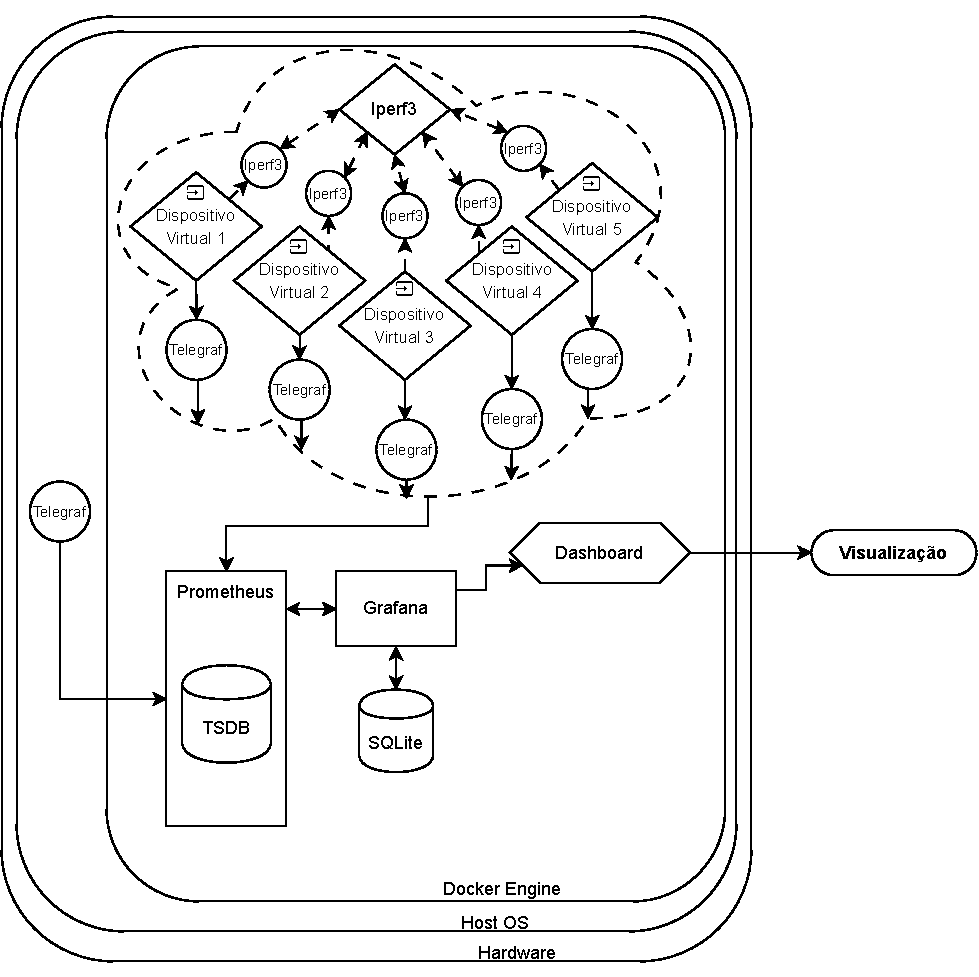
\includegraphics[width=\textwidth]{Imagens/chap04/by-blocks/dashboard_diagram.pdf}
\caption{Visualização.}
\label{fig:DiagramaVisualizacao}
\end{figure}

\begin{figure}[H]
\centering
\color{red}
\setlength{\abovecaptionskip}{-20pt}
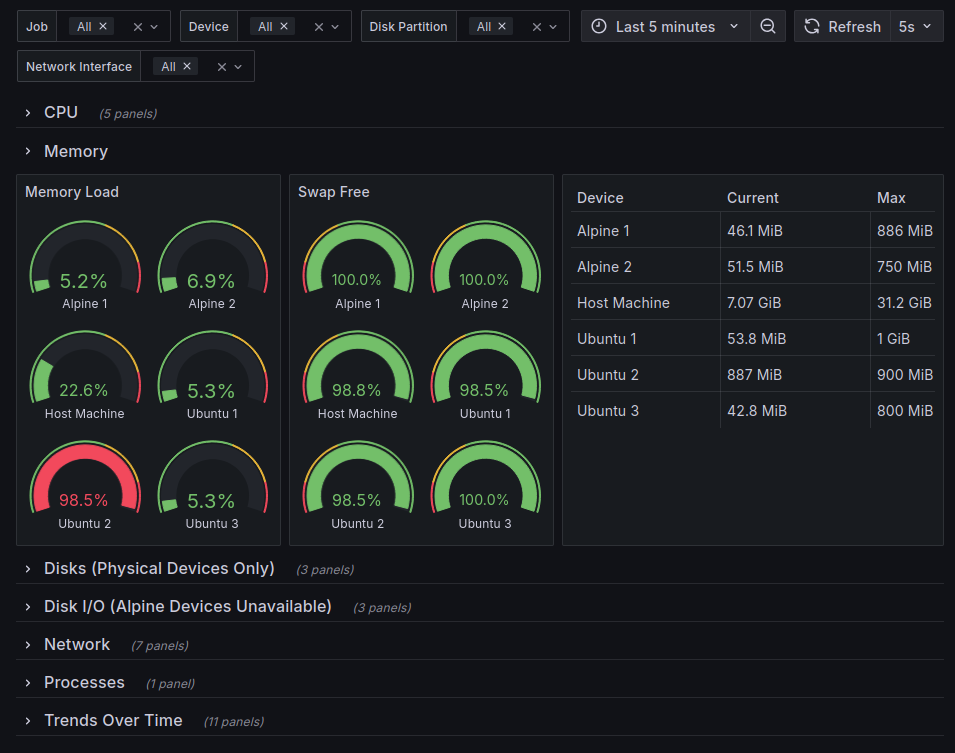
\includegraphics[width=\textwidth]{Imagens/chap04/dashboard/home.png}
\caption{Dashboard - Visão Geral.}
\label{fig:dashboard-home}
\end{figure}

{\color{red}
A Figura \ref{fig:dashboard-home} apresenta a visão geral do dashboard, desenvolvido para fornecer uma representação imediata e concisa do estado de saturação do sistema, permitindo ao usuário identificar rapidamente sinais de saturação elevada. Na parte superior, encontram-se os botões que possibilitam a interação do usuário com os dados. Do canto superior esquerdo até o centro estão as \verb|Grafana Variables|, listadas na Tabela \ref{tab:grafana-variables}, que funcionam como filtros seletivos. Do centro até o canto superior direito, estão localizados os seletores de janelamento histórico e frequência de atualização do dashboard.

O dashboard é organizado em seções horizontais que funcionam como um \foreign{dropdown}, segmentando as informações por categoria de métrica. No exemplo mostrado na Figura \ref{fig:dashboard-home}, a seção \myenquote{Memory} está expandida, exibindo gráficos e visualizações relacionados às métricas de memória coletadas. Esta mesma lógica aplica-se às demais seções, com exceção da seção \myenquote{Trends Over Time}.

Na seção \myenquote{Trends Over Time}, são exibidos gráficos de séries temporais para análise de dados históricos. Diferentemente das outras seções, aqui são apresentadas visualizações de todas as métricas coletadas. Essa ampliação do escopo permite que o usuário realize correlações entre as métricas, facilitando a investigação de problemas, como pode ser observado na Figura \ref{fig:dashboard-timeseries}.

\begin{figure}[H]
\centering
\color{red}
\setlength{\abovecaptionskip}{-20pt}
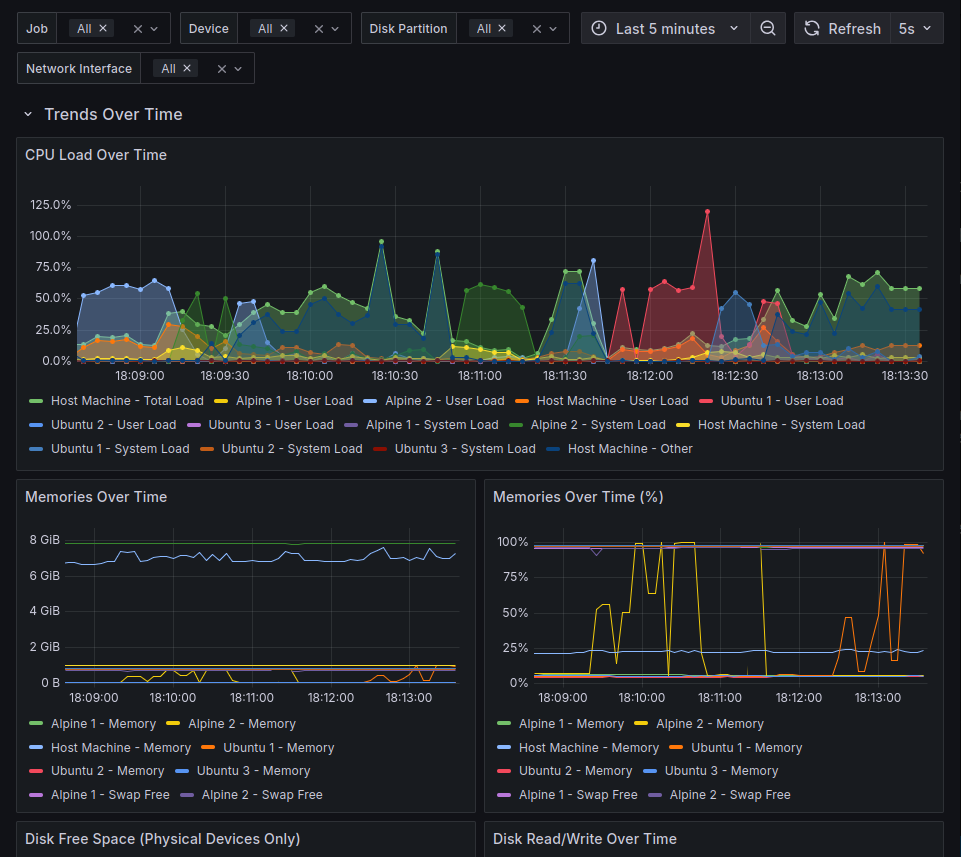
\includegraphics[width=\textwidth]{Imagens/chap04/dashboard/trends_over_time.png}
\caption{Séries Temporais.}
\label{fig:dashboard-timeseries}
\end{figure}

Na seção de CPU, ilustrada na Figura \ref{fig:dashboard-cpu}, 
têm-se gráficos de carga de usuário, carga de sistema, aguardo por I/O, carga total e cargas diversas, específicas de cada dispositivo. No entanto, como apresentado na Tabela \ref{tab:metricas-selecionadas}, algumas métricas não estão presentes em todos os dispositivos, como é o caso da métrica de aguardo por I/O, que não é coletada nos dispositivos virtuais.

Uma observação relevante é que, apesar da métrica de tempo ocioso estar disponível, para contêineres ela sempre apresenta o valor zero, em função da forma como o cgroup gerencia os recursos, impedindo assim o cálculo das métrica de carga total e cargas diversas, que dependem direta e indiretamente do tempo ocioso, respectivamente.

\begin{figure}[H]
\centering
\color{red}
\setlength{\abovecaptionskip}{-20pt}
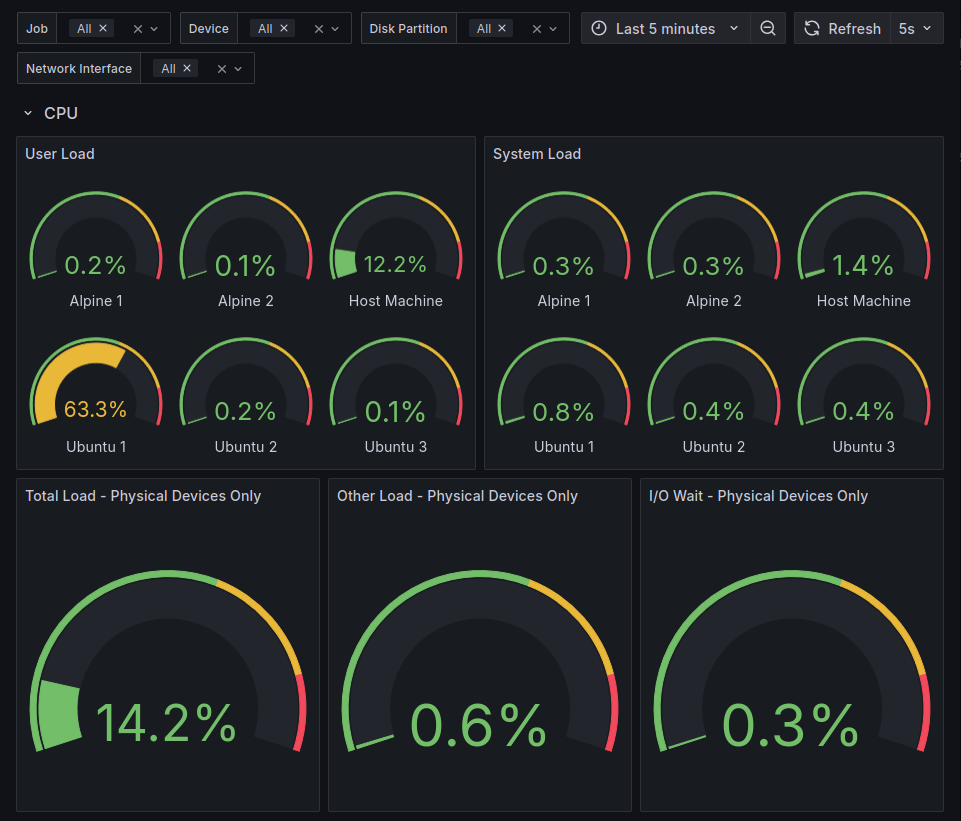
\includegraphics[width=\textwidth]{Imagens/chap04/dashboard/cpu.png}
\caption{Seção de CPU.}
\label{fig:dashboard-cpu}
\end{figure}

Na seção de memórias (ilustrada na Figura \ref{fig:dashboard-memory}), são apresentados gráficos de uso da memória RAM e memória swap disponível, enquanto na seção de Disco I/O (Figura \ref{fig:dashboard-diskio}), encontram-se gráficos de operações de leitura e escrita em disco. Destaca-se que nesta subseção observa-se a indisponibilidade de dados provenientes dos dispositivos Alpine. Isso ocorre devido a uma incompatibilidade entre a definição geral do \verb|inputs.cgroups| do Telegraf e a estrutura de cgroups do Alpine, o que provoca um erro de \foreign{parse} durante a leitura das métricas. Embora uma possível solução seja a criação de um arquivo de configuração específico para o Alpine, decidiu-se não implementá-la. Para fins ilustrativos, foi aplicado o filtro \verb|Device = Host Machine|, que seleciona o dispositivo físico.

\begin{figure}[H]
\centering
\color{red}
\setlength{\abovecaptionskip}{-20pt}
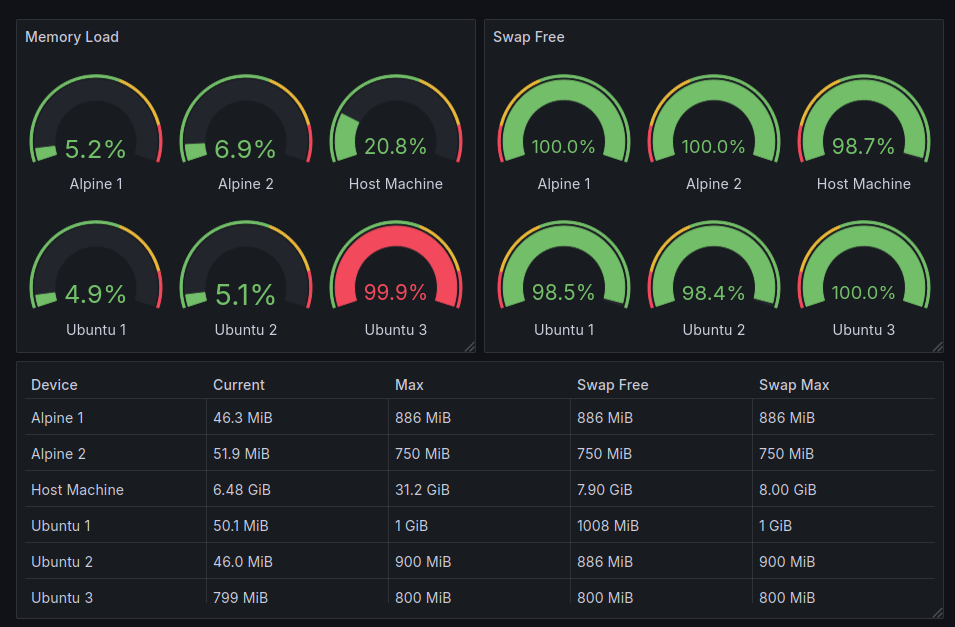
\includegraphics[width=\textwidth]{Imagens/chap04/dashboard/memory.png}
\caption{Seção de Memórias.}
\label{fig:dashboard-memory}
\end{figure}

\vspace{1cm}

\begin{figure}[H]
\centering
\color{red}
\setlength{\abovecaptionskip}{-20pt}
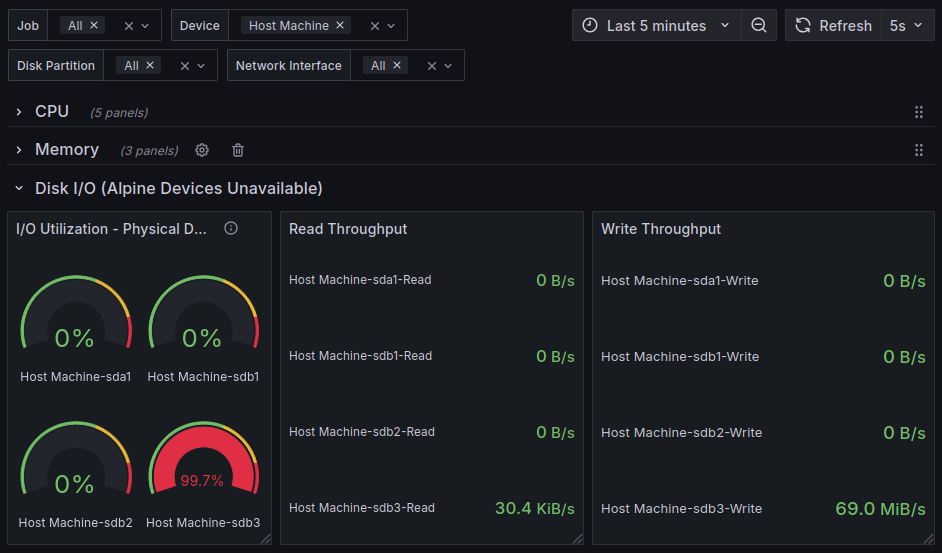
\includegraphics[width=\textwidth]{Imagens/chap04/dashboard/diskio.png}
\caption{Seção de Disco I/O.}
\label{fig:dashboard-diskio}
\end{figure}

Por conta das particularidades das métricas de disco --- como discrepâncias em disponibilidade, optou-se por separar métricas de disco em duas seções: as de leitura e escrita das métricas, apresentadas anteriormente, e as de espaço livre e utilizado em disco, além da quantidade de INODES livres, são apresentadas na seção de Disco (Figura \ref{fig:dashboard-disk}). 

\begin{figure}[H]
\centering
\color{red}
\setlength{\abovecaptionskip}{-20pt}
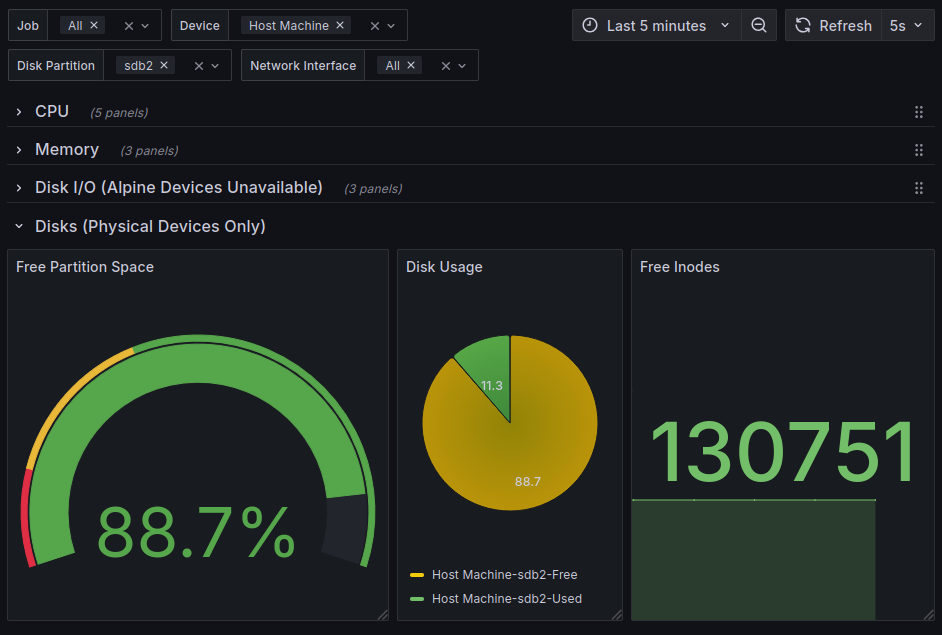
\includegraphics[width=\textwidth]{Imagens/chap04/dashboard/disk.png}
\caption{Seção de Disco.}
\label{fig:dashboard-disk}
\end{figure}

Uma observação importante, embora pouco intuitiva, refere-se à métrica de espaço total em disco. Embora esteja disponível, essa métrica não é a mais adequada para os cálculos dos gráficos. Para determinar o espaço total utilizado, conforme explicitado em nota na documentação do plugin \verb|inputs.disk| \citep{inputsdisk2025}, utiliza-se a soma dos valores de espaço livre e utilizado, descartando-se o valor da métrica de espaço total. Isso ocorre porque a métrica de espaço total reportada pelos sistemas de arquivos pode incluir blocos reservados para o superusuário (\foreign{root}) e outras finalidades do sistema, que não estão disponíveis para usuários comuns, enquanto a soma \myenquote{livre + utilizado} representa de forma mais fiel o espaço efetivamente utilizável.

Para validar a precisão dos dados, realizou-se a comparação entre os valores de espaço livre e utilizado coletados pelo Telegraf e os valores fornecidos pelo comando \verb|df -h| do Linux, uma das ferramentas mais utilizadas para essa finalidade. Os resultados indicaram que os valores obtidos pelo Telegraf apresentaram uma margem de erro inferior a 1\% quando comparados aos valores fornecidos pelo comando \verb|df -h|, provando a confiabilidade das métricas coletadas.

\begin{figure}[H]
\centering
\color{red}
\setlength{\abovecaptionskip}{-20pt}
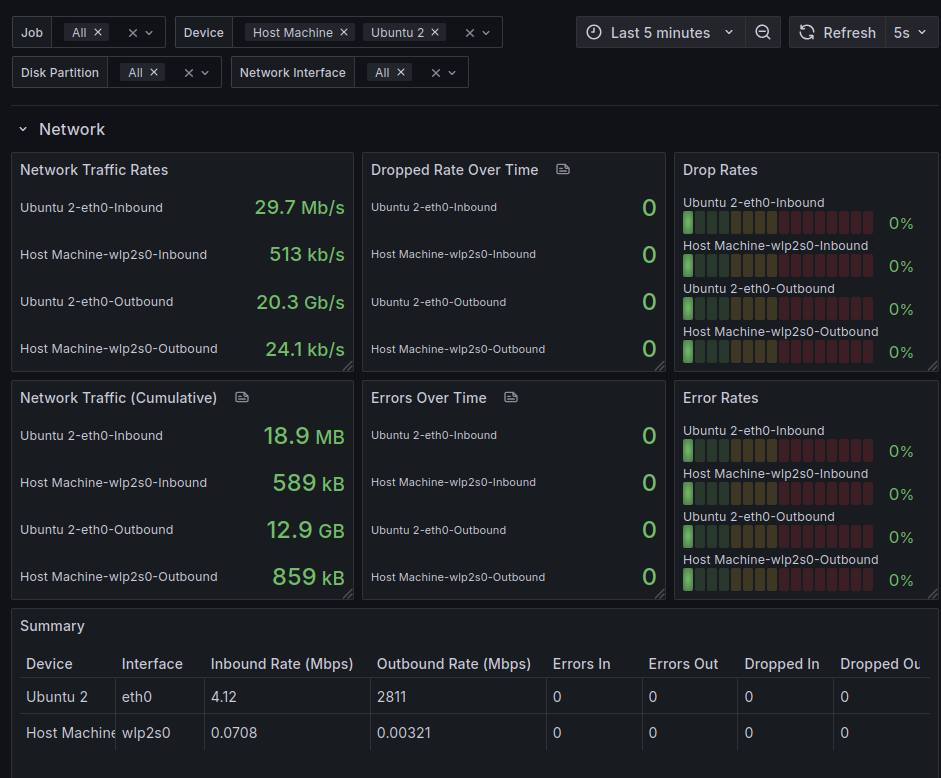
\includegraphics[width=\textwidth]{Imagens/chap04/dashboard/network.png}
\caption{Seção de Rede.}
\label{fig:dashboard-network}
\end{figure}

A Figura \ref{fig:dashboard-network} apresenta a seção de Rede, na qual, mais uma vez para fins ilustrativos, aplicou-se o filtro de dispositivos, nesta ocasião selecionando dos dispositivos \myenquote{Host Machine} e \myenquote{Ubuntu 2}. Essa seção exibe valores instantâneos e acumulativos de tráfego de rede, bem como as quantidades de pacotes descartados ou com erros.

A ausência de dados sobre pacotes descartados ou com erros nos dispositivos virtuais está relacionada à camada de coleta dessas métricas. Tentativas de utilização das ferramentas de \foreign{chaos-engineering} Pumba e ChaosBlade, bem como manipulações diretas no \verb|iptables| para geração de tráfego de rede, mostraram-se inadequadas para este estudo.

Por debaixo dos panos, ferramentas de \foreign{chaos testing} utilizam para testes de rede o módulo \verb|netem| do sistema \verb|tc| do Linux. Esse sistema opera na camada de controle de tráfego (\verb|qdisc|), enquanto o \foreign{plugin} \verb|inputs.net| do Telegraf opera a partir da leitura do \verb|procfs/net/dev|, que se encontra na camada de interface de rede. Por tanto, por estarem em camadas distintas, o Telegraf é incapaz de captar as informações de pacotes descartados ou com erros contabilizados pelo sistema.

\begin{figure}[H]
\centering
\color{red}
\setlength{\abovecaptionskip}{-20pt}
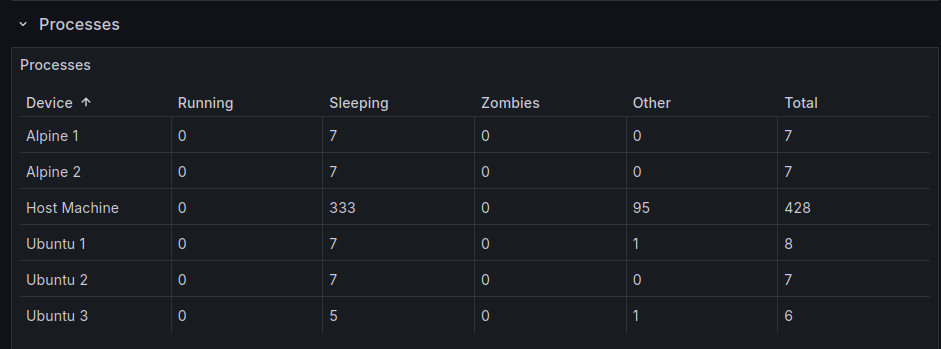
\includegraphics[width=\textwidth]{Imagens/chap04/dashboard/processes.png}
\caption{Seção de Processos.}
\label{fig:dashboard-processes}
\end{figure}

Finalmente, a Figura \ref{fig:dashboard-processes} exibe uma tabela com as quantidades dos processos selecionados, conforme especificado na Tabela \ref{tab:metricas-selecionadas} da Seção \ref{section:DiscussaoMetricas} do capítulo anterior.

Retornando à seção de séries temporais, destacam-se dois gráficos específicos: o uso de CPU e o uso de RAM. Na Figura \ref{fig:dashboard-cpu144}, observa-se que a carga de usuário da CPU no dispositivo virtual 3 ultrapassou 100\%. Embora possa parecer contraditório, visto que na Tabela \ref{tab:EspecificaçõesDispositivosVirtuais} foi estabelecido um limite máximo de utilização de 70\% para um único núcleo de CPU, esse fenômeno decorre das limitações do Docker na imposição de limites de CPU.

Assim, apesar da limitação, a figura evidencia que o contêiner pode apresentar picos de utilização superiores a 100\%, ou seja, utilizar mais de um núcleo de CPU. No caso específico apresentado, o valor de 144\% indica que o contêiner utilizou o equivalente a 1,44 núcleos de CPU.

Por fim, na figura \ref{fig:roundrobin}, observa-se a sequência rotativa de execução dos testes de saturação, conforme detalhado na Seção \ref{subsection:TestesSaturacao}. Essa rotação é evidenciada pelos picos alternados de utilização de memória entre os dispositivos virtuais, demonstrando que os testes foram executados de forma síncrona e sequencial, conforme implementado.

Após o desemvolvimento do \foreign{dashboard}, o mesmo foi exportado em formato JSON e versionado no repositório do projeto \citep{vitorcossetti2025}, na pasta \verb|configs/grafana/dashboards|. A configuração do Grafana foi ajustada para carregá-lo automaticamente via volume Docker, conforme detalhado no Capítulo \ref{chap3}.

\begin{figure}[H]
\centering
\color{red}
\setlength{\abovecaptionskip}{-20pt}
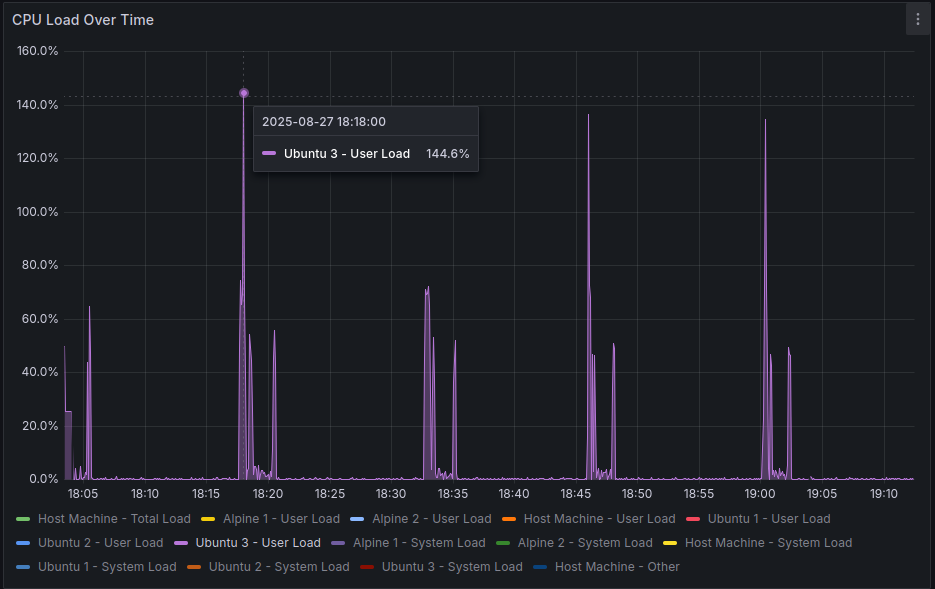
\includegraphics[width=\textwidth]{Imagens/chap04/dashboard/cpu144.png}
\caption{Pico de 144\% de carga de usuário para CPU.}
\label{fig:dashboard-cpu144}
\end{figure}

\begin{figure}[H]
\centering
\color{red}
\setlength{\abovecaptionskip}{-20pt}
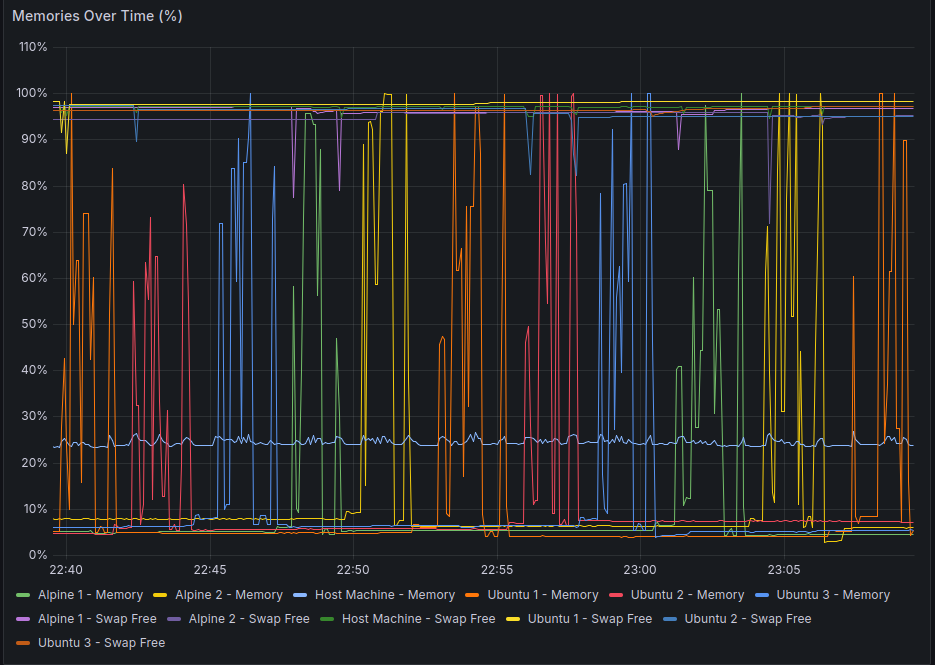
\includegraphics[width=\textwidth]{Imagens/chap04/dashboard/round_robin_sequence.png}
\caption{Sequência rotativa de execução de carga.}
\label{fig:roundrobin}
\end{figure}













\section{Alertas e Notificações}
\label{section:Alertas}

Para o sistema de alertas, inicialmente foram exploradas as funcionalidades nativas do Grafana, que permitem a criação de alertas diretamente na interface web. Essa abordagem inicial foi adotada devido à sua simplicidade e integração direta com os gráficos do dashboard, facilitando a associação visual entre os dados monitorados e os alertas correspondentes.

Como canais de comunicação, foram configurados o envio de e-mails e notificações por aplicativo de mensagens. A configuração do canal de e-mail utilizou o servidor SMTP do Gmail, enquanto a integração com o aplicativo foi realizada por meio da criação de um bot específico para esse propósito. Entretanto, a integração com o aplicativo apresentou desafios técnicos que resultaram em erros, inviabilizando seu uso para notificações, restando somente o canal de e-mail funcional.

Além dos pontos de contato e canais, foram definidas políticas de notificação e regras de alerta baseadas em limiares específicos para as métricas monitoradas. Essas regras foram configuradas para disparar notificações quando determinados parâmetros ultrapassassem valores críticos durante um período estabelecido.

No entanto, essa abordagem apresentou uma limitação crítica. O Grafana, em sua configuração padrão, utiliza o banco de dados SQLite, o que implica que o gerenciamento de alertas, notificações, estados, \foreign{logging} e outros serviços sujeitos a alta frequência de escrita são armazenados em um banco de dados não otimizado para grandes volumes de operações concorrentes. Essa limitação tornou-se evidente quando o sistema passou a apresentar falhas constantes devido a erros de \foreign{database lock}, como \foreign{max-retries-reached}.

Diante dessa criticidade, optou-se pela migração do banco de dados do Grafana para PostgreSQL. Essa migração foi facilitada pela abordagem de IaC adotada, bem como pelo fato de o armazenamento persistente dos dados coletados ficar sob responsabilidade do Prometheus, que já utilizava o TSDB. A migração foi realizada de forma simples, adicionando um contêiner baseado na imagem oficial do PostgreSQL e configurando os parâmetros do Grafana para integração com o novo banco e uso de volumes Docker. Após a migração, o sistema apresentou melhora significativa na estabilidade e no desempenho, eliminando os erros de \foreign{database lock} e permitindo uma gestão mais eficiente dos alertas e notificações.

Entretanto, essa migração evidenciou uma questão arquitetural. A solução inicialmente adotada, embora funcional, introduzia complexidade adicional ao requerer a manutenção de dois bancos de dados distintos: o TSDB do Prometheus e o PostgreSQL do Grafana. Essa complexidade poderia ser evitada com a adoção do Alertmanager, ferramenta nativa do Prometheus para gerenciamento de alertas. O Alertmanager é projetado especificamente para lidar com alertas gerados pelo Prometheus, oferecendo funcionalidades avançadas de roteamento, agrupamento e silenciamento de alertas, além de suporte nativo a múltiplos canais de notificação.

Assim, decidiu-se migrar o sistema de alertas para o Alertmanager, integrando-o diretamente com o Prometheus. A implementação dessa mudança enfrentou alguns desafios, uma vez que o contêiner do Alertmanager, baseado na imagem oficial, apresentava dificuldades na leitura dos arquivos de configuração do projeto. Essas limitações foram superadas mediante a criação de um novo contêiner Alpine customizado, configurado com o Alertmanager e ferramentas essenciais como \verb|curl| e \verb|gettext|, além de um script para automatizar a leitura e validação dos arquivos de configuração em tempo de execução. Apesar da complexidade adicional introduzida para contornar as limitações da imagem oficial, essa solução permitiu uma integração eficiente do Alertmanager com o restante da arquitetura.

Após a integração do Alertmanager, todas as configurações previamente realizadas no Grafana foram migradas sem dificuldades, considerando que ambas as plataformas utilizam arquivos YAML para configuração. Em seguida, realizou-se o \foreign{rollback} do banco de dados do Grafana para SQLite, visando simplificar a arquitetura e reduzir o custo computacional do sistema. Embora com frequência significativamente menor, eventuais falhas de \foreign{database lock} foram novamente detectadas, corroborando a recomendação da literatura contra a utilização do SQLite em cenários de alto volume de escrita concorrente, o que tornou necessário manter o PostgreSQL como SGDB\abbrev{SGDB}{Sistema Gerenciador de Banco de Dados} do Grafana.

Pode-se questionar por que não retornar ao uso do Grafana como gerenciador de alertas, considerando que a manutenção de um banco de dados adicional mostrou-se inevitável e a adição do Alertmanager introduziu complexidade extra. A resposta reside no fato de que, para cada alerta criado no Grafana, uma consulta PromQL percorre todo o fluxo descrito na Seção \ref{section:Dashboard}, podendo aumentar significativamente o custo computacional do sistema, especialmente em ambientes de alta escalabilidade com múltiplos alertas e gráficos. Por outro lado, no Alertmanager, os alertas são gerados diretamente pelo Prometheus, eliminando a necessidade de consultas adicionais e reduzindo o impacto no desempenho do sistema. Portanto, a otimização na execução das regras de alertas justifica o custo do contêiner adicional do Alertmanager.

\begin{figure}[H]
\centering
\setlength{\abovecaptionskip}{-20pt}
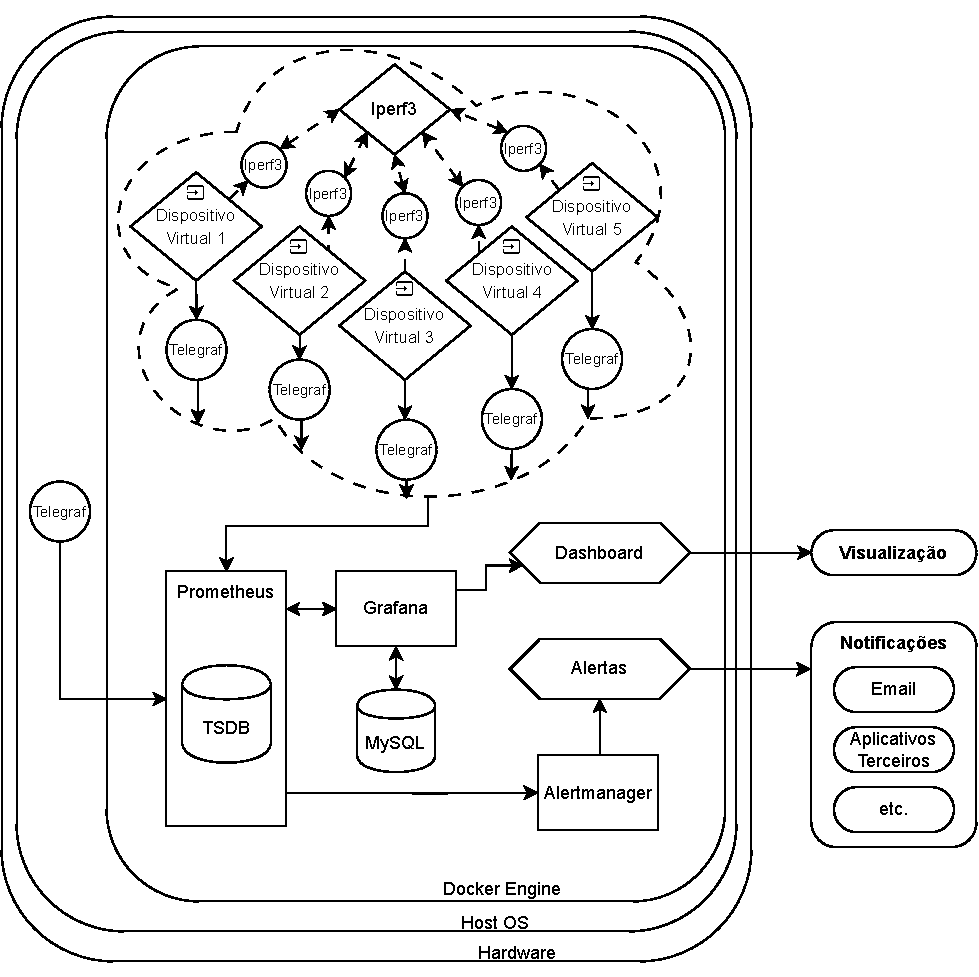
\includegraphics[width=\textwidth]{Imagens/chap04/by-blocks/alerts_diagram.pdf}
\caption{Notificações e Arquitetura Final.}
\label{fig:DiagramaAlertas}
\end{figure}

\begin{figure}[H]
\centering
\setlength{\abovecaptionskip}{-20pt}
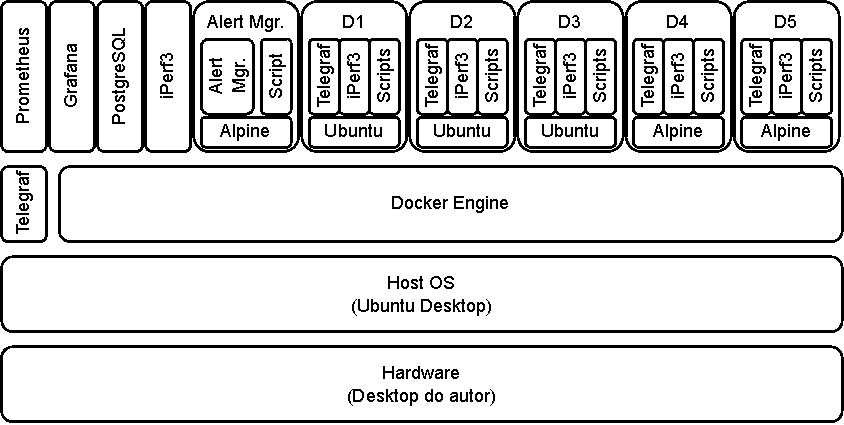
\includegraphics[width=\textwidth]{Imagens/chap04/final_stack.pdf}
\caption{\foreign{Stack} final.}
\label{fig:StackFinal}
\end{figure}









}

\section{Caso de Uso}
\label{section:CasosDeUso}

Um caso de uso para este projeto é o monitoramento da saturação dos equipamentos do próprio autor. Com o dashboard e notificações de alertas desenvolvidos nestre trabalho, foi possível identificar causadores de travamentos, como picos de \myenquote{Aguardo de I/O} da CPU e \myenquote{Utilização I/O} de disco quando executando os testes de saturação dos contêineres de forma assíncrona, o que motivou para a mudança para a execução síncrona dos testes, conforme detalhado em \ref{subsection:TestesSaturacao}.





  %   \chapter{Conclusão}
\label{chap5}

\section{Considerações Finais}
\label{section:ConsideracoesFinais}

Este trabalho atingiu com êxito o objetivo de desenvolver uma plataforma completa de monitoramento de dispositivos, capaz de coletar, armazenar, processar e apresentar visualizações e notificações de dados e métricas pertinentes à observabilidade de saturação de dispositivos. A solução proposta demonstrou eficácia no auxílio à detecção de gargalos sistêmicos e na identificação de oportunidades de otimização. Consequentemente, contribuiu para o aprimoramento do desempenho e da eficiência operacional dos dispositivos monitorados.

A arquitetura adotada, fundamentada em contêineres Docker, revelou-se flexível e escalável. Esta abordagem possibilitou uma implantação simplificada e facilitou a adaptação a diferentes ambientes operacionais. A implementação de paradigmas de Infraestrutura como Código acelerou os processos de configuração, manutenção, replicação, migração e recuperação da plataforma, resultando em redução significativa do tempo e dos recursos necessários para essas operações.

Adicionalmente, a adoção exclusiva de ferramentas de código aberto proporcionou duplo benefício: minimizou os custos associados ao desenvolvimento e operação da plataforma e assegurou elevado grau de personalização dos componentes utilizados. Esta estratégia resultou em maior adaptabilidade da solução às necessidades específicas do contexto de aplicação.

\section{Trabalhos Futuros}
\label{section:TrabalhosFuturos}

A integração de mecanismos de monitoramento para dispositivos móveis representa uma oportunidade significativa de desenvolvimento, especialmente considerando a ausência de suporte oficial para tais dispositivos.

Paralelamente, a implementação da solução em plataformas físicas dedicadas, como dispositivos Intel NUC ou Raspberry Pi, constituiria uma validação importante da viabilidade técnica e comercial da proposta. Tal implementação permitiria avaliar o desempenho em condições reais de operação e forneceria subsídios para o desenvolvimento de um eventual produto comercializável no mercado de IoT.

No contexto do mercado de IoT, o desenvolvimento de módulos específicos para setores industriais e o aprimoramento da adaptabilidade para monitoramento agentless ampliariam significativamente o alcance e a aplicabilidade da plataforma nesses segmentos especializados.

Adicionalmente, a incorporação de funcionalidades de machine learning para análise preditiva e proativa constituiria um importante diferencial competitivo. Tais recursos permitiriam antecipar falhas potenciais e otimizar estratégias de manutenção dos dispositivos monitorados, complementando efetivamente as capacidades reativas atualmente disponíveis.


  %   \chapter{Conclusões}
\label{chap6}

Se chegou aqui é porque você ta quase lá, você vai conseguir, força!!


  \backmatter
  % \nocite{*}
  \bibliographystyle{coppe}
  \bibliography{thesis}
  \addcontentsline{toc}{chapter}{Bibliografia}
  \appendix
  % \chapter{Códigos Fonte dos Dispositivos Virtuais}
\label{apendiceA}

Seção do Docker Compose referente aos dispositivos virtuais.
\begin{lstlisting}[breaklines=true, basicstyle=\small\ttfamily]
services:
# ...
  virtual_device_1:
    container_name: device_1
    build:
      dockerfile: ${UBUNTU_DOCKERFILE}
      context: .
    image: ${UBUNTU_DEVICE_IMG}
    hostname: device1
    cpus: "0.6"
    mem_limit: "1024m"
    networks:
      - devices_network
    volumes:
      - /etc/timezone:/etc/timezone:ro
      - /etc/localtime:/etc/localtime:ro
    healthcheck:
      test: ["CMD", "curl", "-f", "http://localhost:9273/metrics"]
      interval: 30s
      timeout: 10s
      retries: 3

  virtual_device_2:
    container_name: device_2
    build:
      dockerfile: ${UBUNTU_DOCKERFILE}
      context: .
    image: ${UBUNTU_DEVICE_IMG}
    hostname: device2
    cpus: "0.6"
    mem_limit: "900m"
    networks:
      - devices_network
    volumes:
      - /etc/timezone:/etc/timezone:ro
      - /etc/localtime:/etc/localtime:ro
    healthcheck:
      test: ["CMD", "curl", "-f", "http://localhost:9273/metrics"]
      interval: 30s
      timeout: 10s
      retries: 3

  virtual_device_3:
    container_name: device_3
    build:
      dockerfile: ${UBUNTU_DOCKERFILE}
      context: .
    image: ${UBUNTU_DEVICE_IMG}
    hostname: device3
    cpus: "0.7"
    mem_limit: "800m"
    networks:
      - devices_network
    volumes:
      - /etc/timezone:/etc/timezone:ro
      - /etc/localtime:/etc/localtime:ro
    healthcheck:
      test: ["CMD", "curl", "-f", "http://localhost:9273/metrics"]
      interval: 30s
      timeout: 10s
      retries: 3
      
  virtual_device_4:
    container_name: device_4
    build:
      dockerfile: ${ALPINE_DOCKERFILE}
      context: .
    image: ${ALPINE_DEVICE_IMG}
    hostname: device4
    cpus: "0.5"
    mem_limit: "886m"
    networks:
      - devices_network
    volumes:
      - /etc/timezone:/etc/timezone:ro
      - /etc/localtime:/etc/localtime:ro
    healthcheck:
      test: ["CMD", "curl", "-f", "http://localhost:9273/metrics"]
      interval: 30s
      timeout: 10s
      retries: 3
      
  virtual_device_5:
    container_name: device_5
    build:
      dockerfile: ${ALPINE_DOCKERFILE}
      context: .
    image: ${ALPINE_DEVICE_IMG}
    hostname: device5
    cpus: "0.6"
    mem_limit: "750m"
    networks:
      - devices_network
    volumes:
      - /etc/timezone:/etc/timezone:ro
      - /etc/localtime:/etc/localtime:ro
    healthcheck:
      test: ["CMD", "curl", "-f", "http://localhost:9273/metrics"]
      interval: 30s
      timeout: 10s
      retries: 3
# ...
\end{lstlisting}

Dockerfile referente aos dispositivos virtuais Ubuntu (1 à 3):
\begin{lstlisting}[breaklines=true, basicstyle=\small\ttfamily]
FROM ubuntu:24.04

RUN apt update && apt install -y wget stress-ng gnupg curl iperf3

RUN wget -q https://repos.influxdata.com/influxdata-archive_compat.key

RUN echo '393e8779c89ac8d958f81f942f9ad7fb82a25e133faddaf92e15b16e6ac9ce4c influxdata-archive_compat.key' | sha256sum -c && cat influxdata-archive_compat.key | gpg --dearmor | tee /etc/apt/trusted.gpg.d/influxdata-archive_compat.gpg > /dev/null

RUN echo 'deb [signed-by=/etc/apt/trusted.gpg.d/influxdata-archive_compat.gpg] https://repos.influxdata.com/debian stable main' | tee /etc/apt/sources.list.d/influxdata.list

RUN apt update && apt install -y telegraf

COPY configs/telegraf/virtual-devices/telegraf.conf /etc/telegraf/telegraf.conf

COPY scripts/load_simulator.sh /usr/local/bin/load_simulator.sh

RUN chmod +x /usr/local/bin/load_simulator.sh

WORKDIR /

CMD ["/bin/bash", "-c", "/usr/local/bin/load_simulator.sh & telegraf --config /etc/telegraf/telegraf.conf"]
\end{lstlisting}

Dockerfile referente aos dispositivos virtuais Alpine (4 e 5):
\begin{lstlisting}[breaklines=true, basicstyle=\small\ttfamily]
FROM alpine:3.21.3

RUN apk update && apk add --no-cache wget stress-ng gnupg curl bash iperf3

RUN apk add --no-cache ca-certificates procps lm-sensors tzdata iputils 

RUN wget -q https://dl.influxdata.com/telegraf/releases/telegraf-1.29.4_linux_amd64.tar.gz && \
    tar -xzf telegraf-1.29.4_linux_amd64.tar.gz && \
    cp -r telegraf-1.29.4/* / && \
    rm -rf telegraf-1.29.4* && \
    mkdir -p /etc/telegraf

COPY configs/telegraf/virtual-devices/telegraf.conf /etc/telegraf/telegraf.conf

COPY scripts/load_simulator.sh /usr/local/bin/load_simulator.sh

RUN chmod +x /usr/local/bin/load_simulator.sh

WORKDIR /

CMD ["/bin/bash", "-c", "/usr/local/bin/load_simulator.sh & telegraf --config /etc/telegraf/telegraf.conf"]
\end{lstlisting}
\end{document}
